\documentclass[10pt,aspectratio=169]{beamer}

% silence some Metropolis warnings
\usepackage{silence}
\WarningFilter{beamerthememetropolis}{You need to compile with XeLaTeX or LuaLaTeX}
\WarningFilter{latexfont}{Font shape}
\WarningFilter{latexfont}{Some font}

% define custom colors
\usepackage{xcolor}
\definecolor{dark gray}{HTML}{444444}
\definecolor{light gray}{HTML}{777777}
\definecolor{dark red}{HTML}{BB0000}
\definecolor{dark green}{HTML}{00BB00}
\definecolor{RoyalBlue}{cmyk}{1, 0.50, 0, 0}

% configure metropolis
\usetheme[numbering=fraction]{metropolis}
\setbeamercolor{background canvas}{bg=white}
\setbeamercolor{frametitle}{bg=dark gray}
\setbeamercolor{alerted text}{fg=dark red}
\setbeamercolor{item projected}{bg=dark red}
\setbeamercolor{local structure}{fg=dark red}
\setbeamersize{text margin left=0.5cm,text margin right=0.5cm}
\setbeamercovered{transparent=10}

% use thicker lines
\makeatletter
\setlength{\metropolis@titleseparator@linewidth}{1pt}
\setlength{\metropolis@progressonsectionpage@linewidth}{1pt}
\makeatother

% custom bullet points
\setbeamertemplate{itemize item}{\color{dark red}$\blacktriangleright$}
\setbeamertemplate{itemize subitem}{\color{dark red}$\blacktriangleright$}
\setbeamertemplate{itemize subsubitem}{\color{dark red}$\blacktriangleright$}
\newcommand{\custombullet}{{\color{dark red}$\blacktriangleright$}\hspace{0.5em}}


% imports
\usepackage[english]{babel}
\usepackage[utf8]{inputenc}
\usepackage{amsthm}
\usepackage{amssymb}
\usepackage{amsmath}
\usepackage{amsfonts}
\usepackage{mathtools}
\usepackage{mathabx}
\usepackage{stmaryrd}
\usepackage{graphicx}
\usepackage{hyperref}
\usepackage{xfrac}
\usepackage{appendixnumberbeamer}
\usepackage{tabularx}

% check and x marks
\usepackage{pifont}
\newcommand{\cmark}{{\color{dark green}\ding{51}}\hspace{0.3em}}
\newcommand{\xmark}{{\color{dark red}\ding{55}}\hspace{0.5em}}


% use classic font for math
\usepackage[T1]{fontenc} % Needed for Type1 Concrete \usepackage{concmath}
\usefonttheme{serif}
\usefonttheme{professionalfonts}
\usepackage{concmath}
\setbeamerfont{equation}{size=\tiny}



% diagrams
\usepackage{tikz}
\usetikzlibrary{decorations.pathreplacing}

% references
\usepackage[natbibapa]{apacite}
\bibliographystyle{apacite}
\renewcommand{\bibsection}{}

% use ampersands instead of "and" for text citations
\AtBeginDocument{\renewcommand{\BBAB}{\&}}

% possessive cites
\makeatletter
\patchcmd{\NAT@test}{\else \NAT@nm}{\else \NAT@nmfmt{\NAT@nm}}{}{}
\DeclareRobustCommand\citepos
  {\begingroup
   \let\NAT@nmfmt\NAT@posfmt
   \NAT@swafalse\let\NAT@ctype\z@\NAT@partrue
   \@ifstar{\NAT@fulltrue\NAT@citetp}{\NAT@fullfalse\NAT@citetp}}
\let\NAT@orig@nmfmt\NAT@nmfmt
\def\NAT@posfmt#1{\NAT@orig@nmfmt{#1's}}
\makeatother

% spaced-out lists
\newenvironment{wideitemize}{\itemize\addtolength{\itemsep}{10pt}}{\enditemize}
\newenvironment{wideenumerate}{\enumerate\addtolength{\itemsep}{10pt}}{\endenumerate}

% replace footnotes with buttons
\usepackage[absolute,overlay]{textpos}
\newcounter{beamerpausessave}
\newcommand{\always}[1]{
    \setcounter{beamerpausessave}{\value{beamerpauses}}
    \setcounter{beamerpauses}{0}
    \pause
    #1 
    \setcounter{beamerpauses}{\value{beamerpausessave}}
    \addtocounter{beamerpauses}{-1}
    \pause
}
\newcommand{\buttons}[1]{\always{
    \begin{textblock*}{\paperwidth}(0.015\textwidth, 1.022\textheight)
        \scriptsize
        #1
    \end{textblock*}
}}
\newcommand{\appendixbuttons}[1]{\always{
    \begin{textblock*}{\paperwidth}(0.015\textwidth, 1.043\textheight)
        \scriptsize
        #1
    \end{textblock*}
}}
\newcommand{\goto}[2]{\hyperlink{#1}{{\color{dark red}$\smalltriangleright$} #2}\hspace{0.5em}}
\newcommand{\goback}[2]{\hyperlink{#1}{{\color{dark red}$\smalltriangleleft$} #2}\hspace{0.5em}}

% custom appendix
\renewcommand{\appendixname}{\texorpdfstring{\translate{Appendix}}{Appendix}}

% change color of cites and URLs
\let\oldcite\cite
\let\oldcitet\citet
\let\oldcitep\citep
\let\oldcitepos\citepos
\let\oldcitetalias\citetalias
\let\oldcitepalias\citepalias
\let\oldurl\url
\def\cite#1#{\citeaux{#1}}
\def\citet#1#{\citetaux{#1}}
\def\citep#1#{\citepaux{#1}}
\def\citepos#1#{\citeposaux{#1}}
\def\citetalias#1#{\citetaliasaux{#1}}
\def\citepalias#1#{\citepaliasaux{#1}}
\def\url#1#{\urlaux{#1}}
\newcommand*\citeaux[2]{{\color{light gray}\oldcite#1{#2}}}
\newcommand*\citetaux[2]{{\color{light gray}\oldcitet#1{#2}}}
\newcommand*\citepaux[2]{{\color{light gray}\oldcitep#1{#2}}}
\newcommand*\urlaux[2]{{\color{light gray}\oldurl#1{#2}}}
\newcommand*\citeposaux[2]{{\color{light gray}\oldcitepos#1{#2}}}
\newcommand*\citetaliasaux[2]{{\color{light gray}\oldcitetalias#1{#2}}}
\newcommand*\citepaliasaux[2]{{\color{light gray}\oldcitepalias#1{#2}}}

% custom math commands
\DeclareMathOperator*{\argmax}{argmax}
\DeclareMathOperator*{\argmin}{argmin}
\renewcommand{\Pr}{\mathbb{P}}
\newcommand{\E}{\mathbb{E}}
\newcommand{\Var}{\mathbb{V}}
\newcommand{\Cov}{\mathbb{C}}
\newcommand{\overbar}[1]{\mkern 1.5mu\overline{\mkern-1.5mu#1\mkern-1.5mu}\mkern 1.5mu}

% tables
\usepackage{booktabs}
\usepackage{colortbl}
\usepackage{multirow}
\usepackage{makecell}
\arrayrulecolor{dark red}

% custom date
\usepackage{datetime}
\newdateformat{monthyeardate}{\monthname[\THEMONTH] \THEYEAR}

% fix pauses with graphics
\usepackage{../resources/fixpauseincludegraphics}




\newcommand{\vect}[1]{\boldsymbol{\mathbf{#1}}}
\newcommand{\pd}[2]{\frac{\partial{#1}}{\partial{#2}}}
\newcommand{\expect}[2]{\mathbb{E}_{#1}\left[{#2}\right]}
\newcommand{\expectsmall}[2]{\mathbb{E}_{#1}{#2}}
\newcommand{\expectsuper}[3]{\mathbb{E}_{#1}^{#2}\left[{#3}\right]}
\newcommand{\ind}[1]{\mathbbm{1}\left\{{#1}\right\}}
\newcommand{\prob}[1]{\mathbb{P}\left\{{#1}\right\}}
\newcommand{\derivative}[2]{\frac{d{#2}}{d{#1}}}
\newcommand{\cat}[1]{\citeasnoun{#1}}

% title page
\title{What's new in demand estimation?}
\author{Chris Conlon}
\institute{KU Leuven}

\date{Summer 2023}




\begin{document}



%--------------
% TITLE PAGE
\begin{frame}[plain] %
\titlepage
\end{frame}


\section{First: Some Review}

\begin{frame}{What is the goal?}
\small
Consider the multi-product Bertrand problem where firms solve: $\arg \max_{p \in \mathcal{J}_f} \pi_f (\mathbf{p}) = \sum_{j \in \mathcal{J}_f} (p_j - c_j) \cdot q_j(\mathbf{p})$:
\begin{align*}
 0&= q_j(\mathbf{p}) + \sum_{k \in \mathcal{J}_f} (p_k - c_k) \frac{\partial q_{k}}{\partial p_j}(\mathbf{p}) \\
\rightarrow p_j &=q_{j}(\mathbf{p}) \left[-\frac{\partial q_{j}}{\partial p_{j}}(\mathbf{p})\right]^{-1} + c_{j} + \sum_{k \in \mathcal{J}_{f} \setminus j} \left(p_{k}-c_{k}\right) \underbrace{\frac{\partial q_{k}}{\partial p_{j}}(\mathbf{p})\left[-\frac{\partial q_{j}}{\partial p_{j}}(\mathbf{p})\right]^{-1}}_{D_{jk}(\mathbf{p})}\\
p_j(p_{-j}) &= \underbrace{\frac{1}{1+1/\epsilon_{jj}(\mathbf{p})}}_{\text{Markup}} \left[ c_j + \sum_{k \in \mathcal{J}_{f} \setminus j}  (p_k-c_k) \cdot  D_{jk} (\mathbf{p}) \right].
\end{align*}
We call $D_{jk}(\mathbf{p}) = \frac{\frac{\partial q_{k}}{\partial p_j}(\mathbf{p})}{\left| \frac{\partial q_{j}}{\partial p_j}(\mathbf{p}) \right|}$ the \alert{diversion ratio} and $\epsilon_{jj}$ the \alert{own elasticity} and these are the main deliverables.
\end{frame}

\begin{frame}
\frametitle{Starting Point: McFadden and MLE}
Each individual's choice $d_{ij} \in\{0,1\}$ and $\sum_{j \in \mathcal{J}} d_{ij} =1$.\\
Consumers make mutually exclusive and exhaustive choices to maximize (indirect) utility:
\begin{align*}
u_{ij} &= \beta_i \, x_{ij}  + \varepsilon_{ij} \text{ and }
u_{i0} = \varepsilon_{i0}\\
d_{ij} &=1 \text{ IFF } [u_{ij} > u_{ik}\, \forall k \neq j]
\end{align*}
Choices follow a Categorical distribution:
\begin{align*}
(d_{i1},\ldots,d_{iJ},d_{i0}) \sim \text{Categorical} (s_{i1},\ldots,s_{iJ},s_{i0} ) 
\end{align*}
\end{frame}


\begin{frame}
\frametitle{Starting Point: McFadden and MLE}
If we assume that $\varepsilon_{ij}$ is Type I extreme value and $\beta_{\iota} \sim f(\beta_{\iota} \mid \theta)$ (some known parametric distribution) then we can write:
\begin{align*}
s_{ij}(\theta)= \mathbb{P}(d_{ij}=1) = \int \frac{\exp[\beta_{\iota} \, x_j]}{1+\sum_{k \in \mathcal{J}} \exp[\beta_{\iota} \, x_k]}\, f(\beta_{\iota} \mid \theta)\, \partial \beta_{\iota}
\end{align*}
Which gives us the log-likelihood:
 \begin{align*}
 \ell(\theta) = \sum_{i=1}^N \sum_{j \in \mathcal{J} \cup \{0\}} d_{ij} \log s_{ij}(\mathbf{x_i} \mid \theta)
 \end{align*}
 There are a bunch of challenges, not least among which is that the above is \alert{inconsistent} if the integral is evaluated with error that doesn't decrease in $N$.
\end{frame}







\begin{frame}
\frametitle{Starting Point: Moving to Aggregate Data}
If each individual is \alert{exchangable} then ex-ante they have the same choice probabilities: $s_{ij}=s_j$, and the sum of $M$ Categoricals is Multinomial:
\begin{align*}
(q_{1}^{*},\ldots,q_{J}^{*},q_{0}^{*}) \sim \text{Mult} (M, s_{1},\ldots,s_{J},s_{0} ) 
\end{align*}
where $q_{j}^{*}=\sum_{i=1}^M d_{ij}$ is a \alert{sufficient statistic}. 
\begin{itemize}
\item If $M$ gets large enough then $(\frac{q_1}{M},\ldots,\frac{q_J}{M},\frac{q_0}{M})\rightarrow (\mathfrak{s}_1,\ldots,\mathfrak{s}_J,\mathfrak{s}_0)$
 \item Idea: Equate observed market shares to the conditional choice probabilities $(s_1(\mathbf{x_i},\theta),\ldots,s_J(\mathbf{x_i},\theta),s_0(\mathbf{x_i},\theta))$.
\item  Challenges: We probably don't really observe $q_0$ and hence $M$.
\item Introduce idea of market $t$ (otherwise not much data!)
\end{itemize}
\end{frame}




\begin{frame}\frametitle{Lots of papers stop here}
\begin{columns}
\begin{column}{0.3\textwidth}
     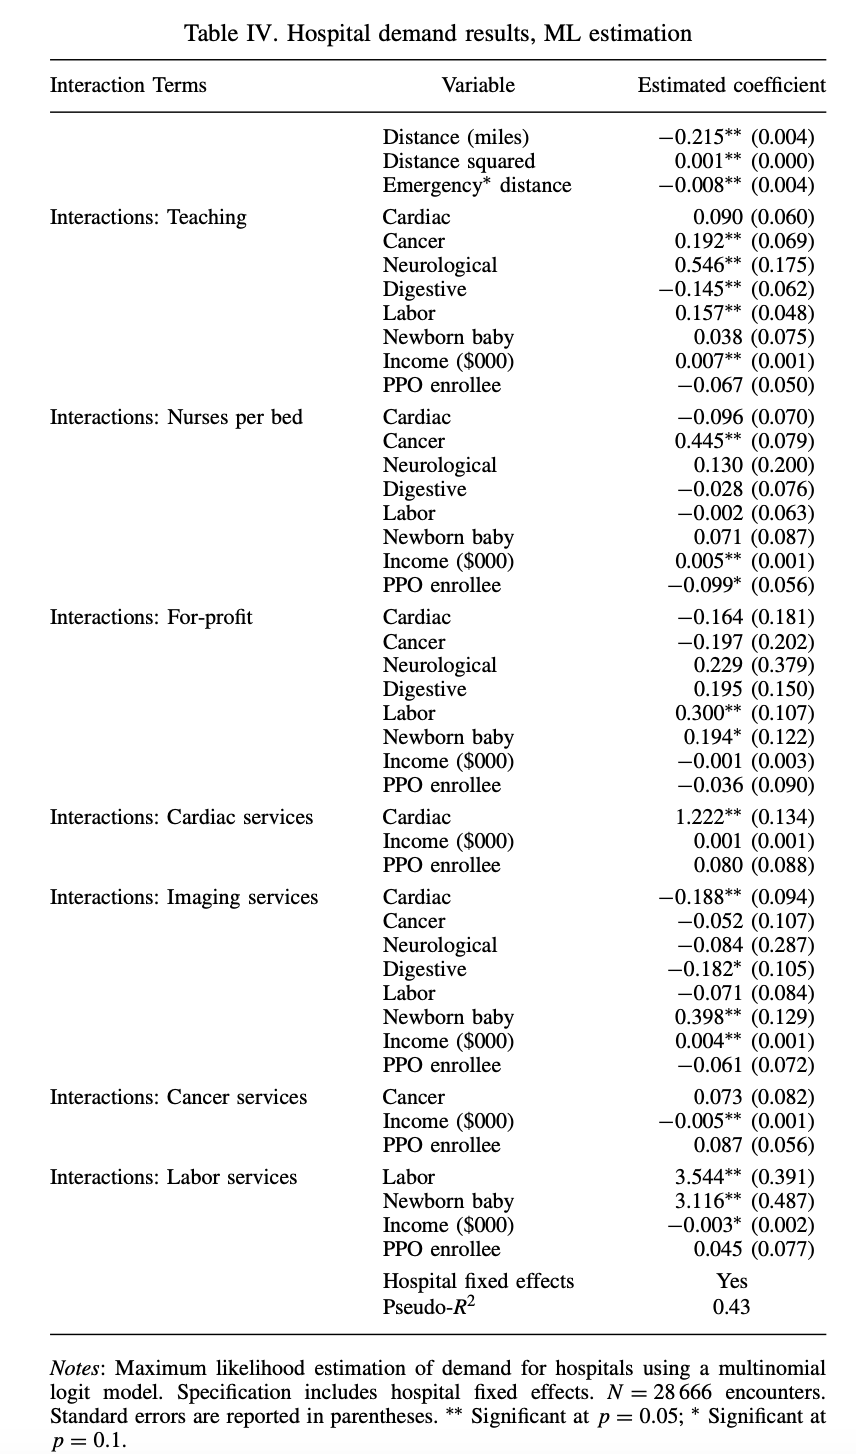
\includegraphics[height=\textheight]{resources/ho_2006}      
\end{column}
\begin{column}{0.7\textwidth}
\begin{itemize}
\item This just MLE on the full individual data from Ho (2006)
\begin{itemize}
\item There is no unobserved heterogeneity, just a deterministic $\beta(y_i)$ where $y_i$ are demographics.
\end{itemize}
\item The ``FTC model'' (Raval, Rosenbaum, Wilson RJE 2022)/ (Raval, Rosenbaum, Tenn EI 2017) groups individuals by income, diagnosis, and zip code and estimates a separate set of $\beta_{g(i)}$ for each group.
\item Hopsitals are a bit special: distance $x_{ij}$ does much of the work (special regressor)
\item Price endogeneity not really a concern (?)
\end{itemize}
\end{column}
\end{columns}
\end{frame}

\begin{frame}{Semiparametric Extensions: Fox Kim Ryan Bajari (QE 2011)}
\vspace{-0.5cm}
\begin{align*}
\nonumber \min_{\pi_i} \sum_{j,t} \left(\mathcal{S}_{jt}(\mathbf{x_t}) - \sum_i \pi_i \cdot s^{*}_{ijt}(\beta^{*}_i, \mathbf{x_t})\right)^2 &
\quad \text{subject to} \quad s^{*}_{ijt}(\beta^{*}_i, \mathbf{x_t}) = \frac{e^{\beta^{*}_i x_{jt} }}{1+\sum_{j'}e^{\beta^{*}_i x_{j't}}}\\
   0\leq  \pi_i \leq 1,& \quad   \sum_i \pi_i = 1
\end{align*}
\vspace{-0.5cm}
\begin{enumerate} 
    \item Draw a large number (thousands?) of $(\beta^{*}_i$ from a prior distribution $g(\beta_i)$ more dispersed than the true $f(\beta_i)$
    \item Compute individual choice probabilities $ s^{*}_{ijt}(\beta^{*}_i)$
    \item Estimate above by constrained least squares (non-negative lasso)
    \item This produces sparse models. (most $\pi_i=0$)
\end{enumerate}
Fixed coefficients require EM. See Heiss, Hetzenecker, Osterhaus (JE 2022) for details (and elastic net variant $\sum_i \pi_i^2 \leq t$).
\end{frame}


\begin{frame}{Applications of Fixed Grid Estimators}
These estimators are helpful when computing choice probabilities is time-consuming (ie: when choices are dynamic). Some recent examples:
\begin{itemize}
    \item Nevo, Turner, Williams (ECMA 2016): Broadband competition
    \item Blundell, Gowrisankaran, Langer (AER 2020): EPA regulation
\end{itemize}
\end{frame}







% % \begin{frame}

% % \end{frame}


% % \begin{frame}
% % \frametitle{Multinomial Logit: Estimation with Aggregate Data}
% % Now suppose we have aggregate data: $(q_1,\ldots,q_J,q_0)$ where $M = \sum_{j \in \mathcal{J}} q_j$.
% % \begin{itemize}
% % \item If $M$ gets large enough then $(\frac{q_1}{M},\ldots,\frac{q_J}{M},\frac{q_0}{M})\rightarrow (\mathfrak{s}_1,\ldots,\mathfrak{s}_J,\mathfrak{s}_0)$
% % \begin{itemize}
% % \item Idea: Observe $(\mathfrak{s}_1(\mathbf{x_i}),\ldots,\mathfrak{s}_J(\mathbf{x_i}), \mathfrak{s}_0(\mathbf{x_i}))$ without sampling variance.
% % \end{itemize}
% % \item Choose $\theta$ that minimizes distance: MLE? MSM? Least Squares? etc.
% % \end{itemize}
% % \end{frame}



\section*{Review: ``Classic'' BLP (1995) Models}
\begin{frame}
\frametitle{Inversion: IIA Logit}
Add unobservable error for each $\mathfrak{s}_{jt}$ labeled $\alert{\xi_{jt}}$.
\begin{align*}
u_{ijt} = \underbrace{x_{jt} \beta -\alpha p_{jt} + \alert{\xi_{jt}}}_{\delta_{jt}} +  \varepsilon_{ijt} , \quad 
\sigma_j(\boldsymbol{\delta_{t}}) = \frac{e^{\delta_{jt}} }{1+\sum_k e^{\delta_{kt}} } 
\end{align*}
\vspace{-0.5cm}
\begin{itemize}
\item The idea is that $\alert{\xi_{jt}}$ is observed to the firm when prices are set, but not to us the econometricians.
\item Potentially correlated with price $\text{Corr}(\xi_{jt},p_{jt}) \neq 0$
\item But not characteristics $\mathbb{E}[\xi_{jt} \mid  x_{jt}]=0$.
\begin{itemize}
\item This allows for products $j$ to better than some other product in a way that is not fully explained by differences in $x_j$ and $x_k$.
\item Something about a BMW makes it better than a Peugeot but is not fully captured by characteristics that leads higher sales and/or higher prices.
\item Consumers agree on its value  (\alert{vertical component}).
\end{itemize}
\end{itemize}
\end{frame}



\begin{frame}
\frametitle{Inversion: IIA Logit}
Taking logs:
\begin{align*}
\ln s_{0t} &= -\log \left(1+\sum_k \exp[x_{kt} \beta + \xi_{kt}] \right) \\
\ln s_{jt} &= [x_{jt} \beta - \alpha p_{jt} +  \xi_{jt} ] - \log \left(1+\sum_k \exp[x_{kt} \beta + \xi_{kt}] \right)\\
\underbrace{\ln s_{jt}- \ln s_{0t}}_{\alert{Data!}} &= x_{jt} \beta -\alpha p_{jt} +  \xi_{jt}
\end{align*}
Exploit the fact that: 
\begin{enumerate}
\item $\ln s_{jt}- \ln s_{0t}= \ln \mathfrak{s}_{jt}- \ln \mathfrak{s}_{0t}$  (with no sampling error)
\item We have one $\xi_{jt}$ for every share $s_{jt}$ (one to one mapping)
\end{enumerate}
\end{frame}



\begin{frame}
\frametitle{Inversion: Nested Logit (Berry 1994 / Cardell 1991)}
This takes a bit more algebra but not much
\begin{align*}
\underbrace{\ln s_{jt}- \ln s_{0t}  - \rho \log(s_{j|gt}) }_{\text{data!}}&= x_{jt} \beta -\alpha p_{jt} +  \xi_{jt} \\
\ln \mathfrak{s}_{jt}- \ln \mathfrak{s}_{0t} &= x_{jt} \beta -\alpha p_{jt} +  \rho \log(\mathfrak{s}_{j|gt})  +  \xi_{jt}
\end{align*}
 \begin{itemize}
\item Same as logit plus an extra term $\log(s_{j|g})$ the \alert{within group share}.
\begin{itemize}
\item We now have a second endogenous regressor.
\item If you don't see it -- realize we are regressing $Y$ on a function of $Y$. This should always make you nervous.
 \end{itemize}
\item If you forget to instrument for $\rho$ you will get $\rho \rightarrow 1$ because of \alert{attenuation bias}.
\item A common instrument for $\rho$ is the number of products within the nest. Why?
 \end{itemize}
\end{frame}

\begin{frame}
\frametitle{BLP 1995/1999 and Berry Haile (2014)}
Think about a \alert{generalized inverse} for $\sigma_{j}(\boldsymbol{\delta_{t}}, \mathbf{x}_t,\theta_2) = \mathfrak{s}_{jt}$ so that 
\begin{align*}
%\sigma_{jt}^{-1}(\mathcal{S}_{\cdot t},\widetilde{\theta}_2)+\alpha p_{jt}&= h(x_{jt},v_{jt},\theta_1)   + \xi_{jt}\\
 \sigma_{jt}^{-1}(\mathcal{S}_{\cdot t},\widetilde{\theta}_2)&= \delta_{jt} \equiv x_{jt} \beta -\alpha p_{jt} +  \xi_{jt} 
\end{align*}
 \begin{itemize}
\item After some transformation of data (shares $\mathcal{S}_{\cdot t}$) we get \alert{mean utilities} $\delta_{jt}$.
% \begin{itemize}
% \item We assume $\delta_{jt}=h(x_{jt},v_{jt},\theta_1) -\alpha p_{jt} + \xi_{jt}$ follows some parametric form (often linear).
%  \end{itemize}
\item Same IV-GMM approach after transformation
\item Examples:
\begin{itemize}
\item Plain Logit: $\sigma_{j}^{-1}(\mathcal{S}_{\cdot t}) = \ln \mathfrak{s}_{jt}- \ln \mathfrak{s}_{0t}$
\item Nested Logit: $\sigma_{j}^{-1}(\mathcal{S}_{\cdot t},\rho) = \ln \mathfrak{s}_{jt}- \ln \mathfrak{s}_{0t} + \rho  \ln \mathfrak{s}_{j|gt}$
\item Three level nested logit: $\sigma_{j}^{-1}(\mathcal{S}_{\cdot t},\rho) = \ln \mathfrak{s}_{jt}- \ln \mathfrak{s}_{0t} +\sum_{d=1}^2 \rho_d \ln \left(\frac{s_{j t}}{s_{d(j), t}}\right)$ (Verboven 1996)
 \end{itemize}
 \item Anything with a share requires an IV (otherwise $\rho \rightarrow 1$).
 \end{itemize}
\end{frame}


\begin{frame}
\frametitle{Aside: Other Analytic Inverses?}
Fosgerau, Monardo, De Palma (2022) propose the IPDL
\begin{align*}
\ln \left(\frac{s_{j t}}{s_{0 t}}\right)=\mathbf{x}_{j t} \boldsymbol{\beta}-\alpha p_{j t}+\sum_{d=1}^D \rho_d \ln \left(\frac{s_{j t}}{s_{d(j), t}}\right)+\xi_{j t}
\end{align*}
 \begin{itemize}
\item Can accomodate multiple (partially) overlapping nests
\item The naive idea (include share within group on RHS with IV) actually works like you would want (!)
\item We need that $\rho > 0$ for this to be RUM.
\item This can allow for mild complementarities as well.
 \end{itemize}
\end{frame}




\begin{frame}
\frametitle{Inversion: BLP}
We can't solve for $\delta_{jt}$ directly this time. We often exploit a trick when $\beta_i,\nu_i$ is normally distributed:
\begin{align*}
\sigma_j(\boldsymbol{\delta_t}; \mathbf{x_t}; \theta_2) &= \int \frac{\exp[\delta_{jt} +  \mu_{ij} ]}{1+\sum_k \exp[\delta_{kt} + \mu_{ik} ]} f(\boldsymbol{\mu_i}| \theta_2)
\end{align*}
 \begin{itemize}
    \item We typically parametrize $\mu_{ijt} = x_{jt} \cdot [\Pi \, y_i + \Sigma \, \nu_{i}]$ where $y_i$ are demographics and $\nu_i$ are unobserved heterogeneity (typically multivariate normal).
    \item Label $\theta_2 = [\Pi, \Sigma, \alpha]$
 \item This is a $J \times J$ system of equations for each $t$.
 \item It is diagonally dominant.
 \item There is a unique vector $\xi_t$ that solves it for each market $t$.
 \end{itemize}
\end{frame}

\begin{frame}
\frametitle{Lots of ways to solve equations (Conlon Gortmaker 2020)}
 \begin{itemize}
     \item If you can work out $\frac{\partial \sigma_{jt}}{\partial \delta_{kt}}$ (easy) you can solve this using Newton's Method. 
 \item BLP prove (not easy) that this is a \alert{contraction mapping}.
\begin{align*}
    \boldsymbol{\delta^{(k)}}(\theta) = \boldsymbol{\delta^{(k-1)}}(\theta) + \log(\mathcal{S}_{j}) - \log(\sigma_{j}(\boldsymbol{\delta_t}^{(k-1)}, \theta)
\end{align*}

\begin{itemize} 
  \item Practical tip: $\epsilon_{tol}$ needs to be as small as possible. ($\approx 10^{-13}$).
 \item Practical tip: Contraction isn't as easy as it looks:  $ \log(\sigma_{j}(\delta_t^{(k-1)}, \theta)$ requires computing the numerical integral each time (either via quadrature or monte carlo).
\end{itemize}
\item We can use \alert{accelerated fixed point} techniques (SQUAREM) (see Reynaerts, Varadhan, and Nash 2012). [PyBLP default].
  \end{itemize}
 \end{frame}


 \begin{frame}
\frametitle{Rewriting as a Convex Program (Li 2018, Monardo 2024)}
We can also solve the following convex program:
\begin{align*}
    \min_{\boldsymbol{\delta}}  \sum_{i=1}^I w_i \cdot \log \left(\sum_{j} \exp\left(\delta_j  + \mu_{ij}(\theta_2) \right) \right) - \sum_k \delta_k \cdot \mathfrak{s}_{k}
\end{align*}
The first-order conditions are given by
$$\sigma_j(\boldsymbol{\delta},\theta_2) = \mathfrak{s}_j$$
And the Hessian requires knowledge of $\frac{\partial \sigma_{j}}{\partial \delta_{k}}$
\begin{itemize}
    \item We are back to solving the non-linear system of equations, but...
    \item Convex programming might be faster/more robust than root finding (why?)
    \item This makes the proof of a unique solution trivial...
  \end{itemize}
 \end{frame}





 \begin{frame}
\frametitle{BLP Pseudocode}
\footnotesize
From the outside, in:
\begin{itemize}
\item Outer loop: search over nonlinear parameters $\theta$ to minimize GMM objective:
 \begin{align*}
 \widehat{\theta_{BLP}} = \arg \max_{\theta} (Z' \hat{\xi}(\theta)) W  (Z' \hat{\xi}(\theta))'
 \end{align*}
 \item Inner Loop:
 \begin{itemize}
% \item Fix $\theta$.
\item Solve for $\delta$ so that $s_{jt}(\delta,\theta) = \tilde{s}_{jt}$.
\begin{itemize}
\item Computing $s_{jt}(\delta,\theta)$ requires numerical integration (quadrature or monte carlo).
\end{itemize}
 \item We can do IV-GMM to recover $\hat{\alpha}(\theta),\hat{\beta}(\theta),\hat{\xi}(\theta)$.
  \begin{align*}
\delta_{jt}= x_{jt} \beta -\alpha p_{jt}+  \xi_{jt}
 \end{align*}
  \item Use $\hat{\xi}(\theta)$ to construct moment conditions.
 \end{itemize}
 \item When we have found $\hat{\theta}_{BLP}$ we can use this to update $W \rightarrow W(\hat{\theta}_{BLP})$ and do 2-stage GMM.
 \end{itemize}
\end{frame}




 \begin{frame}
\frametitle{BLP Estimation}
The model is still defined by CMR $\mathbb{E}[\xi_{jt} \mid  z_{jt}^D]=0$
\begin{itemize}
 \item Now that you have done change of variables to get:
 \begin{align*}
\delta_{jt}= x_{jt} \beta -\alpha p_{jt}+  \xi_{jt}
 \end{align*}
 \item We can do IV-GMM to recover $\hat{\alpha}(\theta_2),\widehat{\beta}(\theta_2),\widehat{\xi}(\theta_2)$.
 \item Outer Loop update guess $\theta$, solve for $\delta$ and repeat.
 \begin{align*}
 \widehat{\theta_{BLP}} = \arg \max_{\theta} (Z' \widehat{\xi}(\theta_2)) W  (Z' \widehat{\xi}(\theta_2))'
 \end{align*}
 \item When we have found $\widehat{\theta_2}_{BLP}$ we can use this to update $W \rightarrow W(\widehat{\theta_2}_{BLP})$ and do 2-stage GMM.
 \end{itemize}
\end{frame}



\begin{frame}
\frametitle{BLP Extensions: Panel Data}
\begin{itemize}
\item with enough observations on the same product it is possible to include fixed effects
\begin{align*}
\delta_{jt}(\theta_2) = x_{jt} \beta - \alpha p_{jt} + \underbrace{\xi_{jt}}_{\xi_{j} + \xi_t + \Delta \xi_{jt}}
\end{align*}
\item What does $\xi_{j}$ mean in this context?
\item What would $\xi_t$ mean in this context?
\item $\Delta \xi_{jt}$ is now the structural error term, this changes our identification strategy a little. 
\begin{itemize}
\item Good: endogeneity problem less severe.
\item Bad: less variation in IV.
\end{itemize}
\end{itemize}
\end{frame}


 \begin{frame}
\frametitle{BLP Alternatives}
\begin{itemize}
 \item BLP give us both a statistical \alert{estimator} and an \alert{algorithm} to obtain estimates.
\item Plenty of other algorithms exist
\begin{itemize}
\item We could solve for $\delta$ using the contraction mapping, using \texttt{fsolve} / Newton's Method / Guess and Check (not a good idea!).
\item We could try and consider a non-nested estimator for the BLP problem instead of solving for $\delta(\theta_2),\xi(\theta_2)$ we could let $\delta,\xi,\alpha,\beta$ be free parameters.
 \end{itemize}
\item We could think about different statistical estimators such as $K$-step GMM, Continuously Updating GMM, etc.
 \end{itemize}
\end{frame}


 \begin{frame}\frametitle{Dube Fox Su (2012)}
\footnotesize
\begin{align}
\label{blpnfxp}
\nonumber \arg \min_{\theta_2} & \psi' \Omega^{-1} \psi \quad \mbox{ s.t. } \\
\nonumber \psi &= \xi(\theta_2)' Z\\
\xi_{jt}(\theta_2) &= \delta_{jt}(\theta_2) - x_{jt} \beta - \alpha p_{jt} \\
\nonumber \log(\mathcal{S}_{jt})  &= \log(\sigma_{jt}(\delta,\theta_2))
\end{align}

\begin{eqnarray}
\label{blpmpec}
\nonumber \arg \min_{\theta_2,\alpha,\beta, \xi,\psi} && \psi' \Omega^{-1}  \psi \quad \mbox{ s.t. } \\
 \psi &=& \xi' Z\\
\nonumber \xi_{jt} &=& \delta_{jt} - x_{jt} \beta - \alpha p_{jt} \\
\nonumber \log(\mathcal{S}_{jt})  &=& \log(\sigma_{jt}(\theta_2, \delta))
\end{eqnarray}
\end{frame}

\begin{frame}
\frametitle{Comparing Approaches}
\begin{itemize}
\item The original BLP paper and the DFS paper define different \alert{algorithms} to produce the same statistical \alert{estimator}.
\begin{itemize}
\item The BLP algorithm is a \alert{nested fixed point} (NFP) algorithm. 
\item The DFS algorithm is a \alert{mathematical program with equilibrium constraints} (MPEC).
\item The unknown parameters satisfy the same set of first-order conditions. (Not only asymptotically, but in finite sample).
\item $\hat{\theta}_{NFP} \approx \hat{\theta}_{MPEC}$ but for numerical differences in the optimization routine.
\end{itemize}
\item Our choice of algorithm should mostly be about computational convenience.
\end{itemize}
\end{frame}

\begin{frame}
\frametitle{BLP: NFP Advantages/Disadvantages}
\begin{itemize}
\item Advantages
\begin{itemize}
\item Concentrate out all of the linear in utility parameters $(\xi,\delta,\beta)$ so that we only search over $\theta_2$. When $\dim(\Sigma)=\theta_2$ is small (few dimensions of unobserved heterogeneity) this is a big advantage. For $K \leq 5$ this is my preferred approach.
\item When $T$ (number of markets/periods) is large then you can exploit solving in parallel for $\delta$ market by market.
\end{itemize}
\item Disadvantages
\begin{itemize}
\item Small numerical errors in contraction can be amplified in the outer loop, $\rightarrow$ tolerance needs to be very tight.
\item Errors in numerical integration can also be amplified in the outer loop $\rightarrow$ must use a large number of draws/nodes.
\item Hardest part is working out the Jacobian via IFT.
%\includegraphics[width=2.8in]{resources/implicit_function.png}\\
\end{itemize}
\end{itemize}
\end{frame}

\begin{frame}
\frametitle{BLP: MPEC Advantages/Disadvantages}
\begin{itemize}
\item Advantages
\begin{itemize}
\item Problem scales better in $\dim(\theta_2)$.
\item Because all constraints hold at the optimum only: less impact of numerical error in tolerance or integration.
\item Derivatives are less complicated than $\frac{\partial \delta}{\partial \theta_2}$ (no IFT).
\end{itemize}
\item Disadvantages
\begin{itemize}
\item We are no longer concentrating out parameters, so there are a lot more of them! Storing the (Hessian) matrix of second derivatives can be difficult on memory $\rightarrow$ Fixed effects are harder
\item We have to find the derivatives of the shares with respect to all of the parameters $\beta,\xi,\theta_2$. (The other derivatives are pretty easy).
\item Parallelizing the derivatives is trickier than NFP case.
\end{itemize}
\end{itemize}
\end{frame}



\section{Adding Supply}
\begin{frame}{Supply}
\begin{itemize}
\item Economic theory gives us some additional powerful restrictions.
\item We may want to impose $MR = MC$.
\item Alternatively, we can ask -- what is a good instrument for demand? \alert{something from another equation} (ie: supply).
\end{itemize}
\end{frame}

\begin{frame}{Some setup}
We can break up the parameter space into three parts:
\begin{itemize}
\item $\theta_1$: linear exogenous demand parameters, 
 \item $\theta_2$: parameters including price and random coefficients (endogenous / nonlinear)
 \item $\theta_3$: linear exogenous supply parameters.
\end{itemize}
\end{frame}



\begin{frame}[plain]
\frametitle{Supply Side}
Consider the multi-product Bertrand FOCs:
\footnotesize
{\begin{align*}
\arg \max_{p \in \mathcal{J}_f} \pi_f (\mathbf{p}) &= \sum_{j \in \mathcal{J}_f} (p_j - c_j) \cdot s_j(\mathbf{p}) +  \kappa_{fg}\sum_{k \in \mathcal{J}_g} (p_k - c_k) \cdot s_k(\mathbf{p}) \\
0&= s_j(\mathbf{p}) + \sum_{k \in \mathcal{J}_f} (p_k - c_k) \frac{\partial s_{k}}{\partial p_j}(\mathbf{p}) 
\end{align*}
}
It is helpful to define the \alert{ownership matrix}:
\begin{align*}
\mathcal{H}(\kappa)_{(j,k)} = \left\{\begin{array}{lr}
          1 & \text{for }  (j,k) \in \mathcal{J}_f \text{ for any } f \\ 
      0 & \text{o.w}\\
        \end{array} \right\}
\end{align*}
We can re-write the FOC in matrix form where $\odot$ denotes Hadamard product (element-wise) and  $\Delta_{(j,k)}(\mathbf{p})  = - \frac{\partial s_{j}}{\partial p_k}(\mathbf{p})$ is the demand derivatives matrix:
\begin{align*}
        s(\mathbf{p}) &= (\mathcal{H} \odot \Delta(\mathbf{p})) \cdot (\mathbf{p} - \mathbf{mc}), \\
       \mathbf{mc} &=  \mathbf{p} - \underbrace{(\mathcal{H} \odot \Delta(\mathbf{p}))^{-1} s(\mathbf{p})}_{\eta(\mathbf{p},\mathbf{s},\theta_2)}.
\end{align*}
\end{frame}



\begin{frame}{Recovering Marginal Costs }
Recover implied markups/ marginal costs, and assume a functional form for $mc_{jt}(x_{jt},w_{jt})$.
\begin{align*}
\mathbf{mc}(\theta)&= \mathbf{p}- \boldsymbol{\eta}(\mathbf{p},\mathbf{s},\theta_2)\\
f(mc_{jt}) &= [\textrm{x}_{jt} \,, \textrm{w}_{jt}] \theta_3 + \omega_{jt}
\end{align*}
Which we can solve for $\omega_{jt}$:
\begin{align*}
\omega_{jt} &=  f(\mathbf{p}- \boldsymbol{\eta}(\mathbf{p},\mathbf{s},\theta_2) ) -[\textrm{x}_{jt} \,, \textrm{w}_{jt}] \theta_3 
\end{align*}
\begin{itemize}
\item $f(\cdot)$ is usually $\log(\cdot)$ or identity.
\item We can use this to form additional moments: $\E[\omega_{jt} \mid  z_{jt}^{s}]=0$.
\item We can just stack these up with the demand moments $E[\xi_{jt}' Z_{jt}^d]=0$.
%\item Now I have $\dim(Z^d) + \dim(Z^s)$ moments altogether.
\item This step is optional but can aid in identification (if you believe it).
\end{itemize}
\end{frame}


\begin{frame}{Additional Details}
Some different definitions:
\begin{alignat}{3}
\label{eq:stacked}
\nonumber y_{jt}^D &:= \widehat \delta_{jt}(\theta_2) + \alpha p_{jt} &=(\textrm{x}_{jt} \-\ \textrm{v}_{jt})' \beta + \xi_t &=: x_{jt}^{D\prime}\beta + \xi_{jt} \\ 
y_{jt}^S &:= \widehat{mc}_{jt}(\theta_2) &= (\textrm{x}_{jt} \-\ \textrm{w}_{jt})'\gamma + \omega_t &=: x_{jt}^{S\prime} \gamma + \omega_{jt} 
\end{alignat}
Stacking the system across observations yields:
\begin{align}
\underbrace{\begin{bmatrix} y_D \\ y_S \end{bmatrix}}_{2N\times1} = 
\underbrace{\begin{bmatrix}
X_D & 0 \\
0 & X_S 
\end{bmatrix}}_{2N\times(K_1+K_3)}
\underbrace{\begin{bmatrix}
\beta \\ \gamma %\Gamma_D \\ \Gamma_S
\end{bmatrix}}_{(K_1+K_3)\times1} + 
\underbrace{\begin{bmatrix}
\xi \\ \omega % \varepsilon_D \\ \varepsilon_S
\end{bmatrix}}_{2N\times 1}
\end{align}
\end{frame}



\begin{frame}{Simultaneous Supply and Demand: in details}
\footnotesize
\begin{enumerate}[(a)]
\item For each market $t$: solve $\mathcal{S}_{jt} = \sigma_{jt}(\delta_{\cdot t},\theta_2)$ for $\widehat{\delta}_{\cdot t}(\theta_2)$.
\item For each market $t$: use $\widehat{\delta}_{\cdot t}(\theta_2)$ to construct $\eta_{\cdot 
t}(\mathbf{q_t},\mathbf{p_t},\widehat{\delta}_{\cdot t}(\theta_2),\theta_2)$
\item For each market $t$: Recover $\widehat{mc}_{jt}(\widehat{\delta}_{\cdot t}(\theta_2),\theta_2) = p_{jt} - \eta_{jt}(\widehat{\delta}_{\cdot t}(\theta_2),\theta_2)$
\item Stack up $\widehat{\delta}_{\cdot t}(\theta_2)$ and $\widehat{mc}_{jt}(\widehat{\delta}_{\cdot t}(\theta_2),\theta_2)$ and use linear IV-GMM to recover $[\widehat{\theta}_1(\theta_2), \widehat{\theta}_3(\theta_2) ]$ following the recipe in Appendix of Conlon Gortmaker (2020)
\item Construct the residuals:
\begin{align*}
\nonumber    \widehat{\xi}_{jt}(\theta_2) &= \widehat{\delta}_{jt}(\theta_2) -  x_{jt} \widehat{\beta}(\theta_2) + \alpha p_{jt}\\
    \widehat{\omega}_{jt}(\theta_2) &= \widehat{mc}_{jt}(\theta_2) -  [x_{jt}\, w_{jt}]\, \widehat{\gamma}(\theta_2)
\end{align*}
\item Construct sample moments
\begin{align*}
\nonumber g_n^D(\theta_2)=\frac{1}{N} \sum_{jt} Z_{jt}^{D\prime} \widehat{\xi}_{jt}(\theta_2)\\
 g_n^S(\theta_2)=\frac{1}{N} \sum_{jt} Z_{jt}^{S \prime} \widehat{\omega}_{jt}(\theta_2)
\end{align*}
\item Construct GMM objective $Q_n(\theta_2)= \left[ {\begin{array}{c} g_n^d(\theta_2) \\ g_n^s(\theta_2) \end{array} } \right]' W  \left[ {\begin{array}{c} g_n^d(\theta_2) \\ g_n^s(\theta_2) \end{array} } \right] $
\end{enumerate}
\end{frame}


\begin{frame}{What's the Point (Conlon Gortmaker RJE 2020)}
\begin{itemize}
\item A well-specified supply side can make it easier to estimate $\theta_2$ parameters (price in particular).
\item Imposing the supply side only helps if we have information about the marginal costs / production function that we would like to impose
\item May want to enforce some economic constraints: ($mc_{jt} > 0$ is a good one).
\item But assuming the wrong conduct $\mathcal{H}_t$ can lead to misspecification!
\end{itemize}
\begin{center}
\includegraphics[width=0.75\textwidth]{resources/supply_table}
\end{center}
\end{frame}



\begin{frame}{What about Misspecification? (Conlon Gortmaker RJE 2020)}
\begin{center}
\includegraphics[height=0.9\textheight]{resources/supply_figure}
\end{center}
\end{frame}

\section*{Quick Case Study}



\begin{frame}{What's the point?}
\begin{align*}
       \mathbf{mc} &=  \mathbf{p} - \eta(\mathbf{p},\mathbf{s},\theta_2).
\end{align*}
Demand systems have two main deliverables:
\begin{itemize}
\item Own-price elasticities $\epsilon_{jj}(\mathbf{p},\theta_2)$
\item Substitution patterns (all transforms of same object)
\begin{itemize}
\item Demand Derivatives: $\Delta(\mathbf{p},\theta_2)$
\item Cross elasticities: $\epsilon_{jk}(\mathbf{p}) = \frac{\partial q_k}{\partial p_j}$
\item Diversion Ratios: $D_{jk}(\mathbf{p}) = \frac{\partial q_k}{\partial p_j}/|\frac{\partial q_j}{\partial p_j}|$
\end{itemize}
\item Other checks: $D_{j0}(\mathbf{p})$ diversion to outside good; $\epsilon^{agg}$ category elasticity to 1\% tax.
\begin{itemize}
    \item Tend to give insight into the economics of the problem.
\end{itemize}
\end{itemize}
\end{frame}



\begin{frame}{Why does supply matter? (Conlon Rao 2014/2023)}
Consumer $i$ chooses product $j$ (brand-size-flavor) in quarter $t$:
\begin{align*}
u_{ijt} &= \beta_{i}^0 -  \alpha_i\, p_{jt} + \beta_i^{1750}\, \cdot \mathbb{I}[1750mL]_j + \gamma_j + \gamma_t+ \varepsilon_{ijt}(\rho)\\
\begin{pmatrix}
\ln \alpha_i\\
\beta_i
\end{pmatrix} &=
\begin{pmatrix}
\overline{\alpha}\\
\theta_1
\end{pmatrix} + \Sigma \cdot \nu_i + \sum_{k} \Pi_k \cdot \mathbb{I}\{LB_k \leq \text{Income}_i < UB_k\} 
\end{align*}
\begin{itemize}
\item Nesting Parameter $\rho$: Substitution within category (Vodka, Gin, etc.) %(Vodka/Tequila/Rum/Gin/Whiskey)
\item Consumers of different income levels have different mean values for coefficients
\item Conditional on income, normally distributed unobserved heterogeneity for:
\begin{itemize}
\item Price $\alpha_i$
\item Constant $\beta_{i}^0$ (Overall demand for spirits)
\item Package Size: $\beta_{i}^{1750}$ (Large vs. small bottles)
\end{itemize}
\end{itemize}
\end{frame}


\begin{frame}{Wholesale Margins Under Post and Hold}
\begin{columns}[T]
\begin{column}{.5\textwidth}
\begin{center}
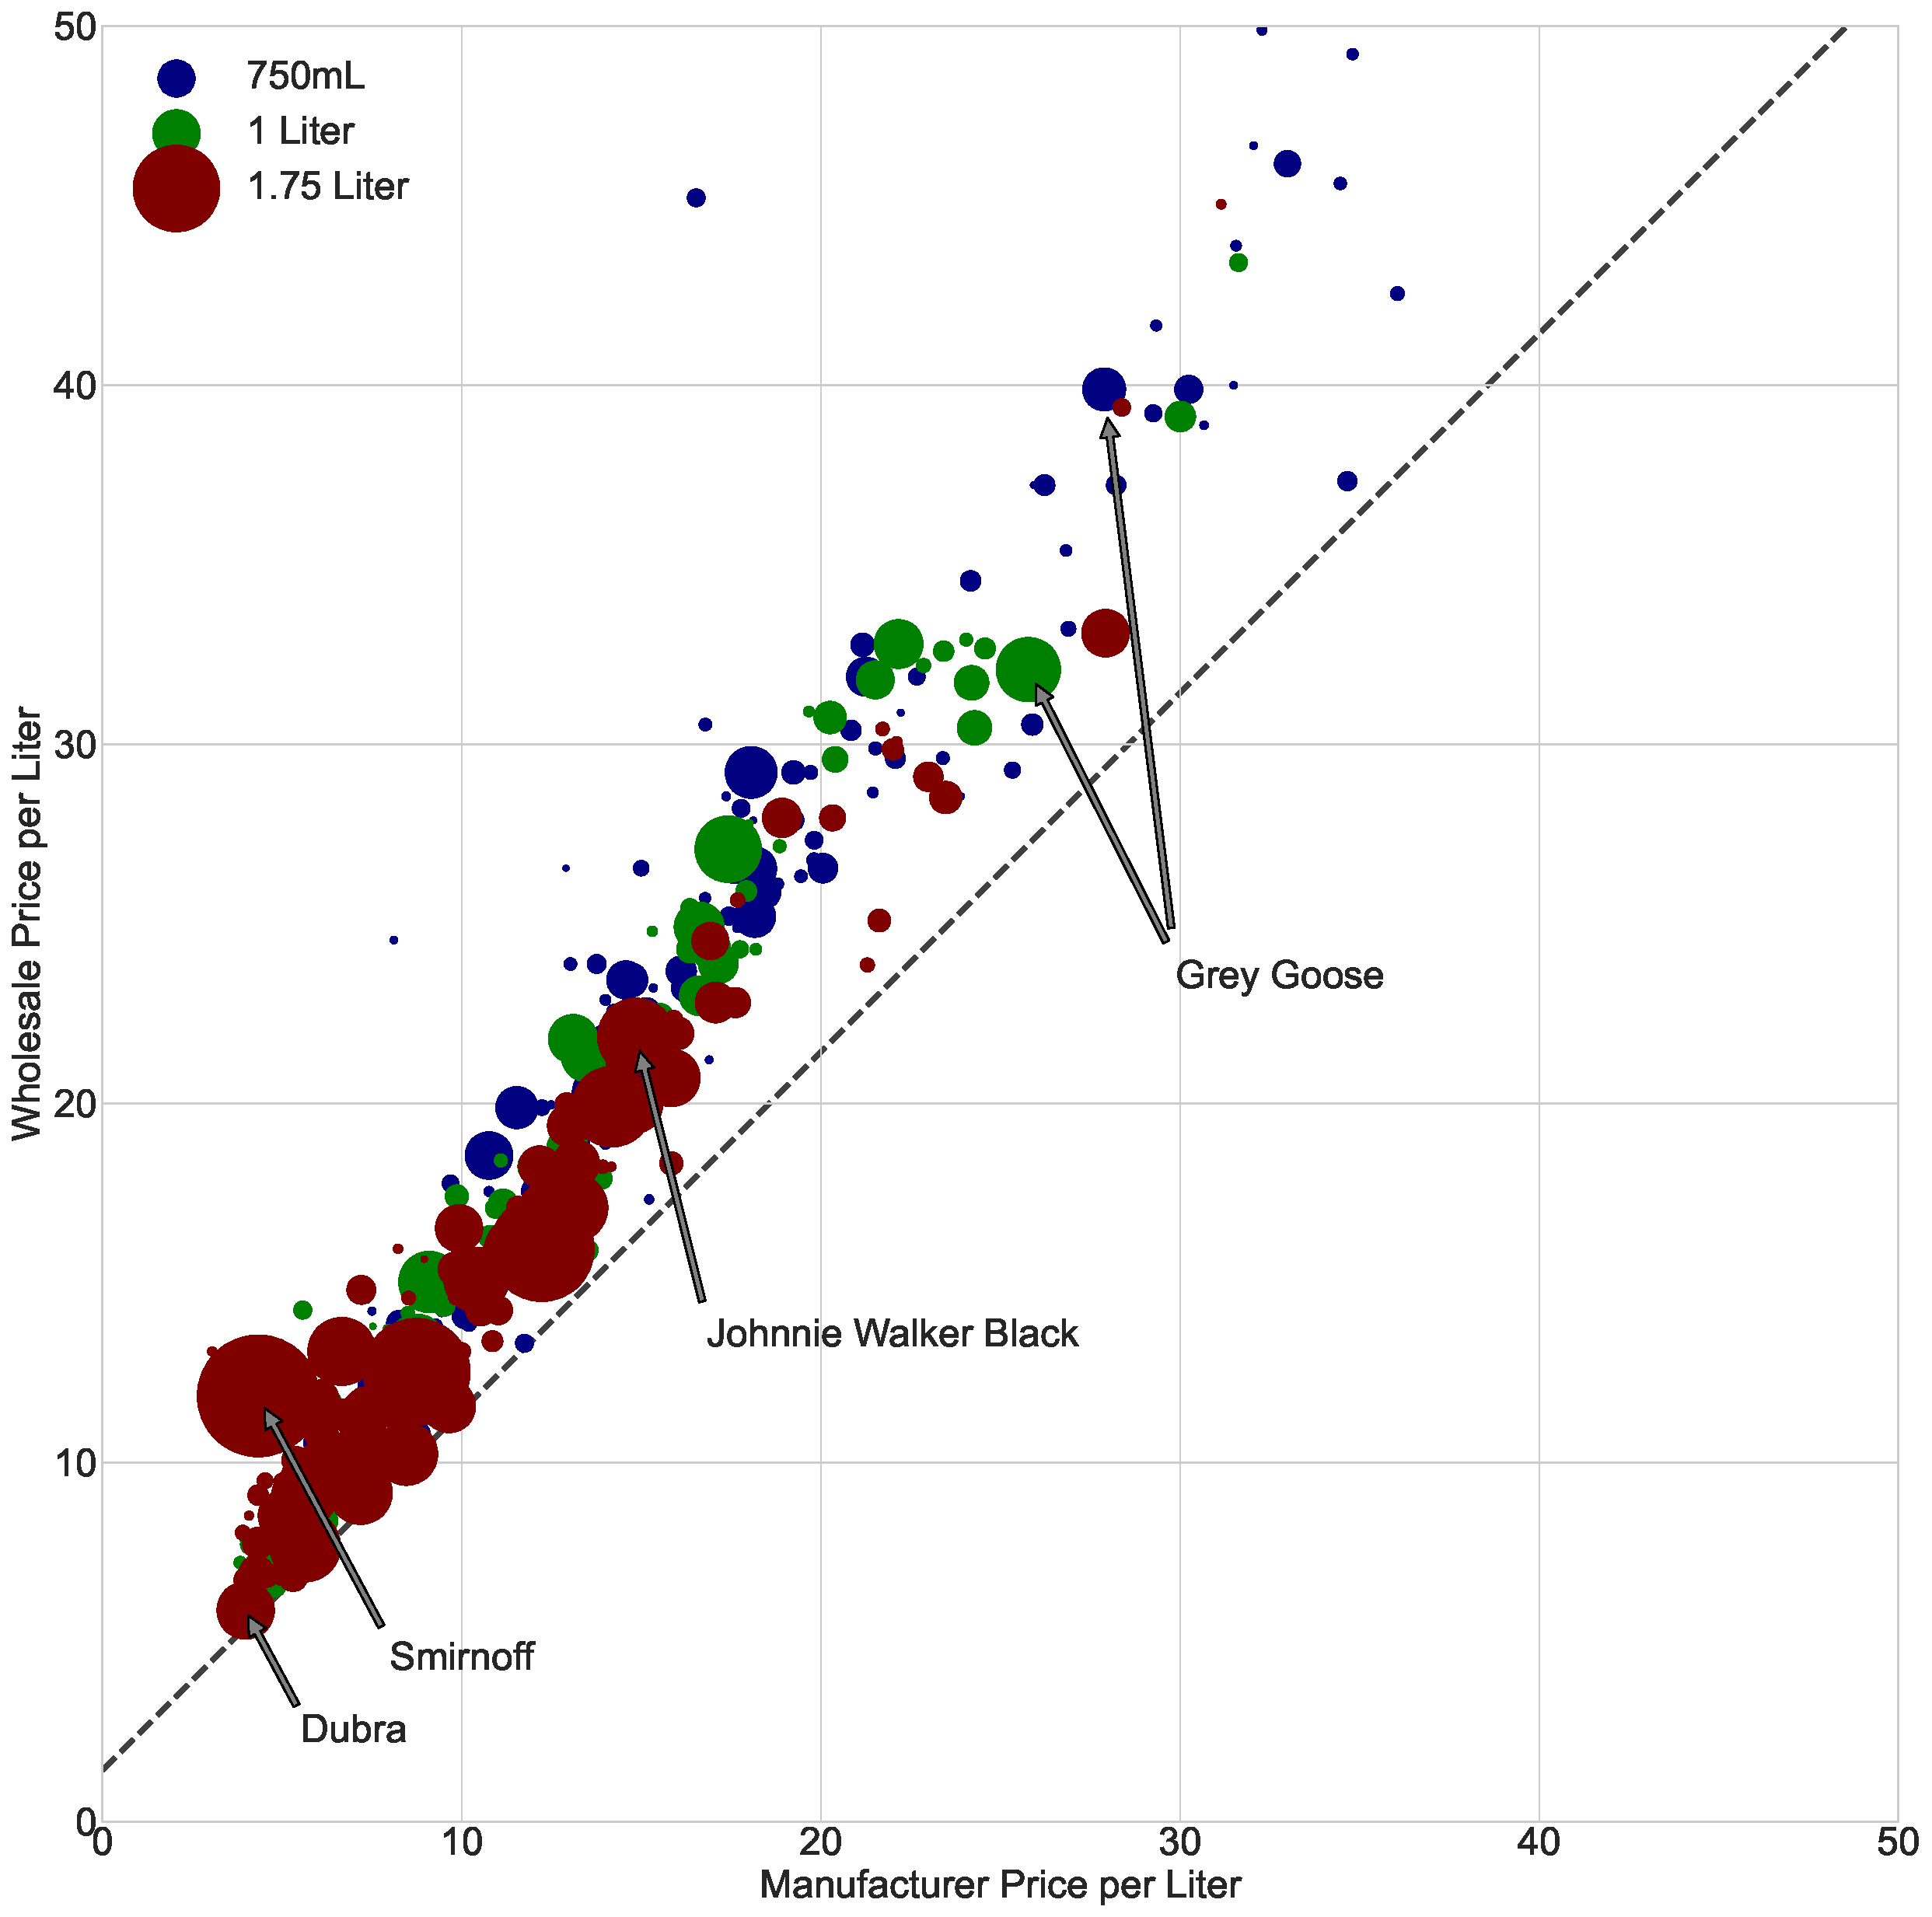
\includegraphics[height=0.88\textheight]{resources/figure4_manuf_wholesale_price.pdf}
\end{center}
\end{column}
\hfill
\begin{column}{.5\textwidth}
  \begin{itemize}
  \item Price Cost Margins (and Lerner Markups) are higher on premium products
  \item Markups on least expensive products (plastic bottle vodka) are very low.
  \item Smirnoff (1.75L) is best seller\\ (high markup / outlier).
  \item A planner seeking to minimize ethanol consumption would flatten these markups!
  \item Matching this pattern is kind of the whole ballgame !
  \item Plain logit gives $\epsilon_{jj} = \alpha \cdot p_j  \cdot (1-s_j)$.
  \end{itemize}
  \end{column}
\end{columns}
\end{frame}



\begin{frame}{Demand Estimates (from \texttt{PyBLP}, Conlon Gortmaker (2020, 2023))}
\begin{columns}[T]
 \hspace{-1.5cm}
 \begin{column}{.68\textwidth}
\vspace{-0.3cm}
    \begin{center}
    \scalebox{0.55}{
    \begin{tabular}{lccc} 
\toprule 
\multicolumn{1}{c}{$\Pi$} &  Const &  Price &  1750mL \\ 
\cmidrule(r){1-1} \cmidrule(rrr){2-4} 
Below \$25k  &  2.928 & -0.260 &   0.543 \\
            &  (0.233) &  (0.056) &   (0.075) \\
\$25k-\$45k   &  0.184 & -0.170 &   0.536 \\
            &  (0.236) &  (0.054) &   (0.083) \\
\$45k-\$70k   &  0.000 & -0.179 &   0.980 \\
            &  (0.000) &  (0.053) &   (0.093) \\
\$70k-\$100k  & -0.452 & -0.496 &   0.608 \\
            &  (0.227) &  (0.051) &   (0.079) \\
Above \$100k & -1.777 & -1.543 &   0.145 \\
            &  (0.234) &  (0.047) &   (0.055) \\
\midrule \multicolumn{1}{c}{$\Sigma^2$}& \multicolumn{2}{c}{} \\ \cmidrule(r){1-1} \cmidrule(rrr){2-4}
Constant    &   1.167 & 0.695   &  \\
            &  (0.236)&(0.048) &   \\
Price       &   0.695 & 0.697  \\
            &   (0.048) &(0.028) \\
\midrule  
\multicolumn{1}{l}{Nesting Parameter $\rho$} &  &0.423&    \\ 
& &(0.026)&     \\ 
\multicolumn{1}{l}{Fixed Effects} &   \multicolumn{3}{c}{Brand+Quarter}\\ 
\midrule 
%\multicolumn{1}{c}{}& \multicolumn{3}{c}{Model Predictions} \\ 
\multicolumn{1}{c}{Model Predictions}& 25\% & 50\% & 75\% \\ \midrule\midrule
Own Elasticity:  $\frac{\partial \log q_j}{\partial \log p_j}$                  & -5.839 & -5.162 & -4.733 \\
Aggregate Elasticity: $\frac{\partial \log Q}{\partial \log P}$            & -0.333 & -0.329 & -0.322 \\
Own Pass-Through: $\frac{\partial p_j}{\partial c_j}$          & 1.256 & 1.284 &  1.320 \\
Observed Wholesale Markup (PH)  &  0.188 &  0.233 &  0.276 \\
Predicted Wholesale Markup (PH) &  0.205 &  0.231 &  0.259 \\
\bottomrule 
\end{tabular}
    }
    \end{center}
  \end{column}
  \hfill
 \hspace{-2.2cm}
\begin{column}{.55\textwidth}
  \begin{itemize}
    \item Demographic Interactions w/ 5 income bins \\ (matched to micro-moments)
    \item Correlated Normal Tastes: (Constant, Large Size, Price)
    \item Supply moments exploit observed upstream prices and tax change (ie: match observed markups).
    \vspace{-0.2cm}
    \begin{align*}
    \mathbb{E}[\omega_{jt}]=0, \text{ with }\omega_{jt} = \left(p^w_{jt}  - p^m_{jt}-\tau_{jt} \right) -\eta_{jt}\left(\theta_2\right).
    \end{align*}
   \vspace{-0.8cm}
   \item Match re-purchase rate of $Vodka \rightarrow Vodka$ for each category.
    \item Pass-through consistent with estimates from our AEJ:Policy paper.
  \end{itemize}
\end{column}
\end{columns}
\end{frame}

\begin{frame}{Elasticities and Diversion Ratios}
\begin{center}
    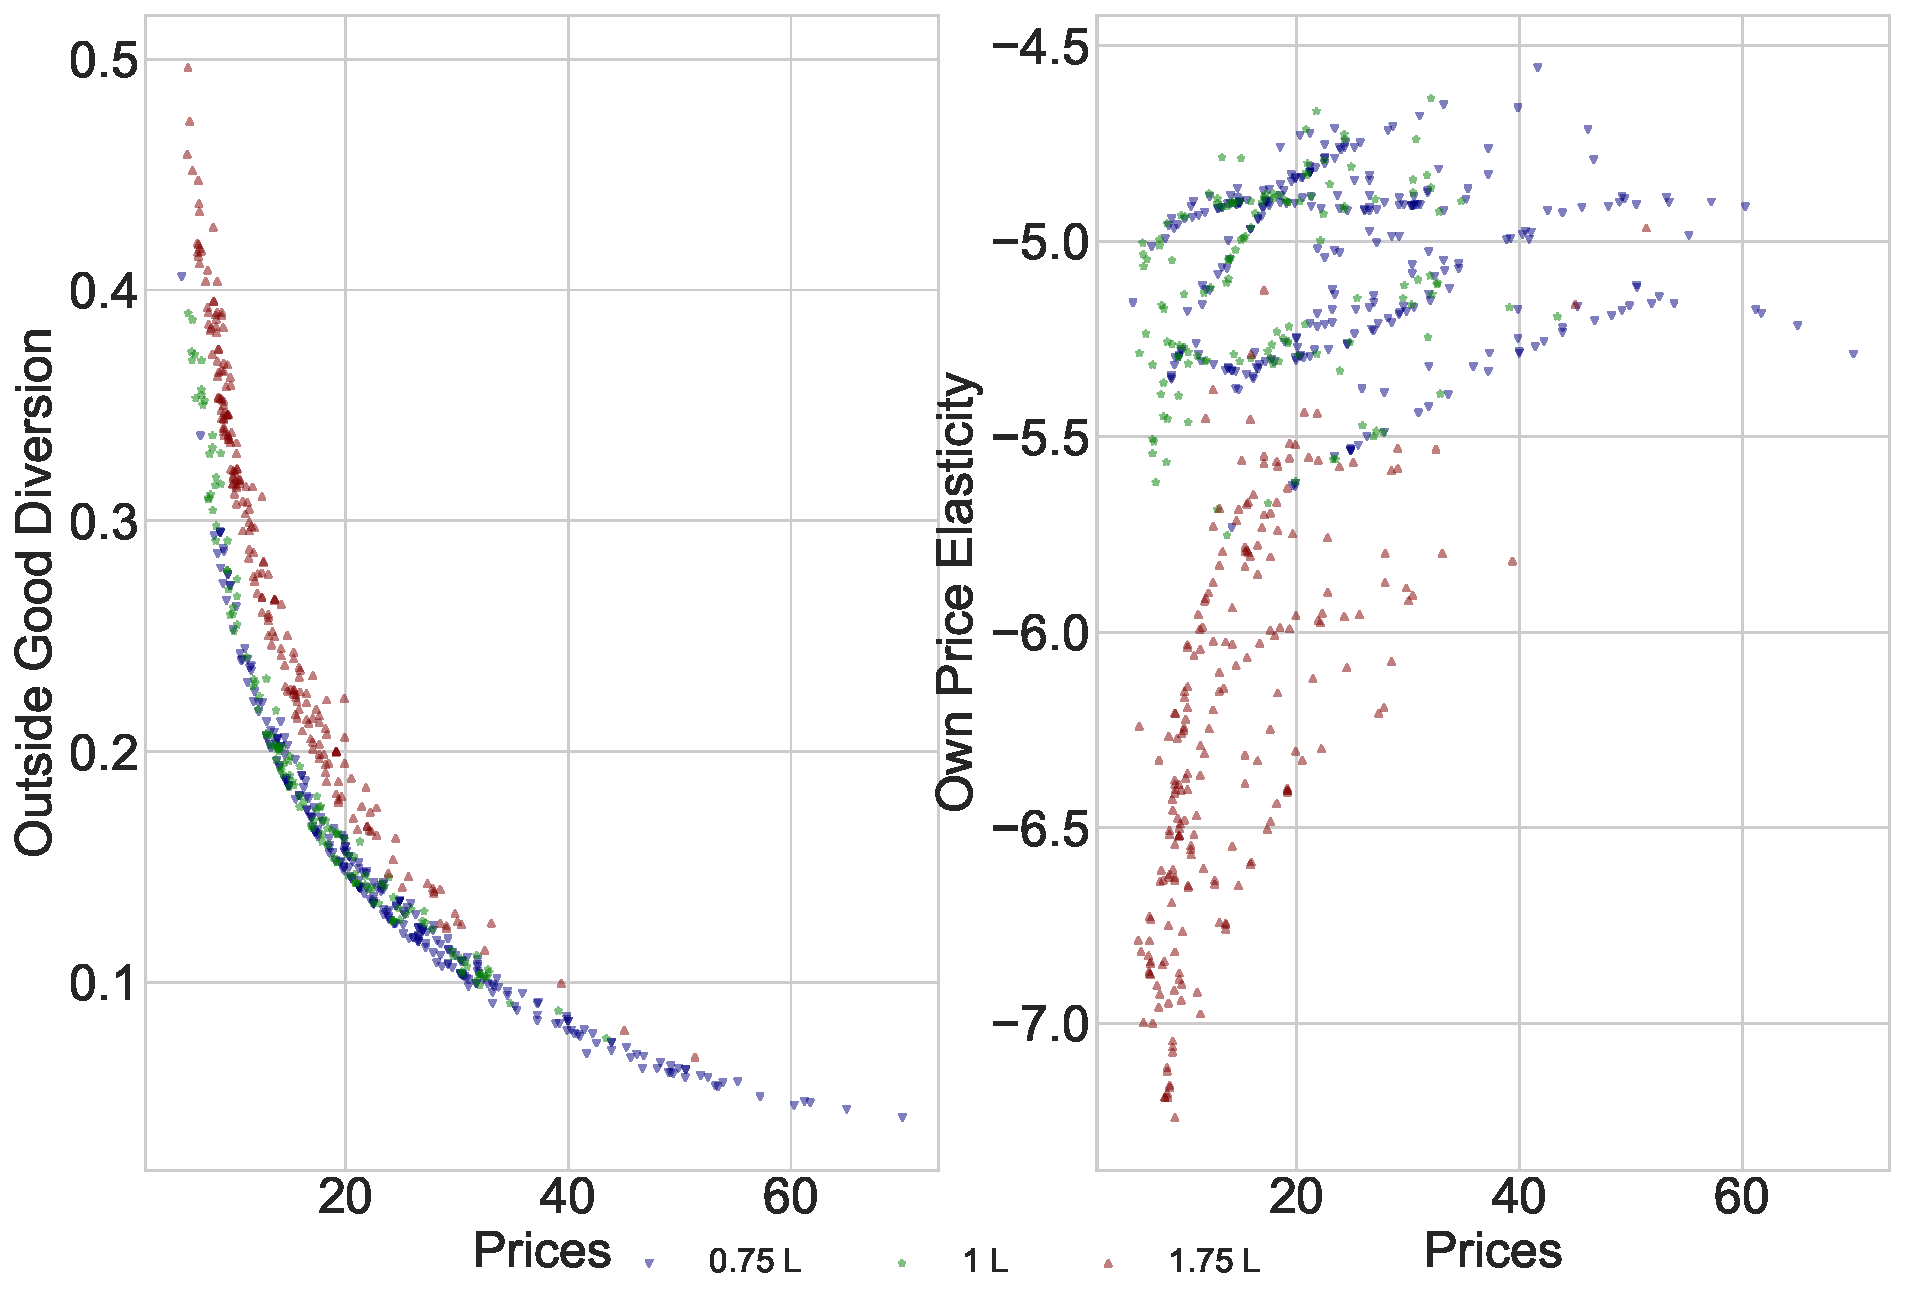
\includegraphics[height=0.95\textheight]{./resources/figure6_outside_diversion_elas_v2.pdf}
\end{center}
\end{frame}



\begin{frame}{Diversion Ratios}
\begin{center}
\scalebox{0.6}{
\begin{tabular}{lrrlrr} 
\toprule 
{}&  Median Price &  \% Substitution &  {}&  Median Price &  \% Substitution \\ 
\midrule 
\multicolumn{1}{c}{Capt Morgan Spiced 1.75 L (\$15.85)} & \multicolumn{5}{c}{ Cuervo Gold 1.75 L (\$18.33) } \\ \cmidrule(lr){1-1} \cmidrule(lrr){4-6} 
\midrule 
        Bacardi Superior Lt Dry Rum 1.75 L & 12.52 & 13.07 &                    Don Julio Silver 1.75 L & 22.81 & 5.00 \\
                   Bacardi Dark Rum 1.75 L & 12.52 &  2.71 &                          Cuervo Gold 1.0 L & 21.32 & 3.82 \\
         Bacardi Superior Lt Dry Rum 1.0 L & 15.03 &  2.44 &              Sauza Giro Tequila Gold 1.0 L &  8.83 & 3.07 \\
                           Smirnoff 1.75 L & 11.85 &  2.36 &                            Smirnoff 1.75 L & 11.85 & 2.44 \\
     Lady Bligh Spiced V Island Rum 1.75 L &  9.43 &  2.18 &                       Absolut Vodka 1.75 L & 15.94 & 2.06 \\
\midrule 
\multicolumn{1}{c}{Woodford 0.75 L (\$34.55)} & \multicolumn{5}{c}{ Beefeater Gin 1.75 L (\$17.09) } \\ \cmidrule(lr){1-1} \cmidrule(lrr){4-6} 
\midrule 
             Jack Daniel Black Label 1.0 L & 27.08 & 7.66 &                           Tanqueray 1.75 L & 17.09 & 12.80 \\
            Jack Daniel Black Label 1.75 L & 21.85 & 4.91 &                             Gordons 1.75 L & 11.19 &  4.14 \\
            Jack Daniel Black Label 0.75 L & 29.21 & 4.83 &                        Seagrams Gin 1.75 L & 10.23 &  2.85 \\
                         Makers Mark 1.0 L & 32.79 & 4.52 &                              Bombay 1.75 L & 21.95 &  2.27 \\
                        Makers Mark 0.75 L & 31.88 & 2.80 &                            Smirnoff 1.75 L & 11.85 &  2.27 \\
\midrule 
\multicolumn{1}{c}{Dubra Vdk Dom 80P 1.75 L (\$5.88)} & \multicolumn{5}{c}{ Belvedere Vodka 0.75 L (\$30.55) } \\ \cmidrule(lr){1-1} \cmidrule(lrr){4-6} 
\midrule 
                        Popov Vodka 1.75 L &  7.66 & 7.56 &                           Grey Goose 1.0 L & 32.08 & 5.09 \\
                           Smirnoff 1.75 L & 11.85 & 3.15 &                       Absolut Vodka 1.75 L & 15.94 & 3.82 \\
                    Sobieski Poland 1.75 L &  9.09 & 3.14 &                        Absolut Vodka 1.0 L & 24.91 & 2.74 \\
                 Grays Peak Vdk Dom 1.75 L &  9.16 & 2.87 &                            Smirnoff 1.75 L & 11.85 & 2.43 \\
                        Wolfschmidt 1.75 L &  6.92 & 2.48 &                          Grey Goose 0.75 L & 39.88 & 2.22 \\
\bottomrule 
\end{tabular}
}
\end{center}
% \begin{tablenotes}
% \item Note: The table above reports diversion rates for five popular products.  Per liter wholesale prices are reported for 2013Q2. We compute the diversion ratio for a small price change $D_{j \rightarrow k} = \frac{\partial q_{k}}{\partial q_{j}}/\left|\frac{\partial q_{j}}{\partial q_{j}}\right|$. Substitutes maintain the same product category but differ across products due to the nesting parameter and random coefficients incorporated in the RCNL model.
% \item A plain logit would predict the best substitute as the product with the largest overall share: Smirnoff Vodka (80 Proof, 1.75L) with $s_{jt} = 1.2\%$ or $4.38\%$ of ``inside'' sales.
% \item Source: Authors' calculations
% \end{tablenotes}
\end{frame}


\section{Instruments and Identification}

\begin{frame}{Parametric Identifcation}
\begin{itemize}
\item Once we have $\delta_{jt}(\theta)$ identification of linear parameters $\theta_1=[\beta,\xi_j, \xi_t]$ is pretty straightforward
\begin{eqnarray*}
\delta_{jt}(\theta) = x_{jt} \beta - \alpha p_{jt} + \xi_j + \xi_t + \Delta \xi_{jt}
\end{eqnarray*}
\item This is either basic linear IV or panel linear IV.
\item Intuition: How are $\theta_2$ taste parameters identified?
\begin{itemize}
\item Consider increasing the price of $j$ and measuring substitution to other products $k,k'$ etc.
\item If sales of $k$ increase with $p_j$ and $(x_j^{(1)},x_k^{(1)})$ are similar then we increase the $\theta_2$ that corresponds to $x^{(1)}$.
\item Price is the most obvious to vary, but sometimes this works for other characteristics (like distance).
\item Alternative: vary the set of products available to consumers by adding or removing an option.
\end{itemize}
\end{itemize}
\end{frame}




\begin{frame}{Instruments}
\begin{itemize}
\item Recall the nested logit, where there are two separate endogeneity problems
\begin{itemize}
\item \alert{Price}: this is the familiar one!
\item \alert{Nonlinear characteristics/Shares} $\theta_2$ this is the other one.
\end{itemize}
\item We are doing nonlinear GMM: Start with $\E[\xi_{jt} | x_{jt}, z_{jt}]=0$ use $\E[\xi' [Z X]]=0$.
\begin{itemize}
\item In practice this means that for valid instruments $(x,z)$ any function $f(x,z)$ is also a valid instrument $\E[ \xi_{jt} f(x_{jt},z_{jt})]=0$.
\item We can use $x, x^2, x^3,\ldots$ or interactions $x \cdot z, x^2 \cdot z^2, \ldots$.
\item What is a reasonable choice of $f(\cdot)$?
\item Where does $z$ come from?
\end{itemize}
\end{itemize}
\end{frame}



\begin{frame}{Exclusion Restrictions (see Berry Haile 2014)}
\begin{eqnarray*}
    \delta_{jt}(\mathcal{S}_t,\alert{\textrm{y}_t}, \widetilde{\theta}_2) &=&  [\textrm{x}_{jt}, \alert{\textrm{v}_{jt}}]  \beta  - \alpha p_{jt} + \xi_{jt}\\
    f(p_{jt} - \eta_{jt}(\theta_2,\mathbf{p},\mathbf{s})) &=&   h(\textrm{x}_{jt},\alert{\textrm{w}_{jt}};\theta_3)+\omega_{jt}
\end{eqnarray*}
The first place to look for exclusion restrictions/instruments:
\begin{itemize}
\item Something in another equation!
\item $\textrm{v}_j$ shifts demand but not supply
\item $\textrm{w}_j$ shifts supply but not demand
\item $\textrm{y}_t$ is a sneaky demand shifter
\item If it doesn't shift either is it really relevant?
\end{itemize}
Alternative: MacKay Miller (2022) propose $Cov(\xi_{jt},  \omega_{jt})=0$ as an alternative.
\end{frame}



\begin{frame}{Cost Shifters Really Matter (from Conlon Gortmaker RJE)}
\begin{center}
    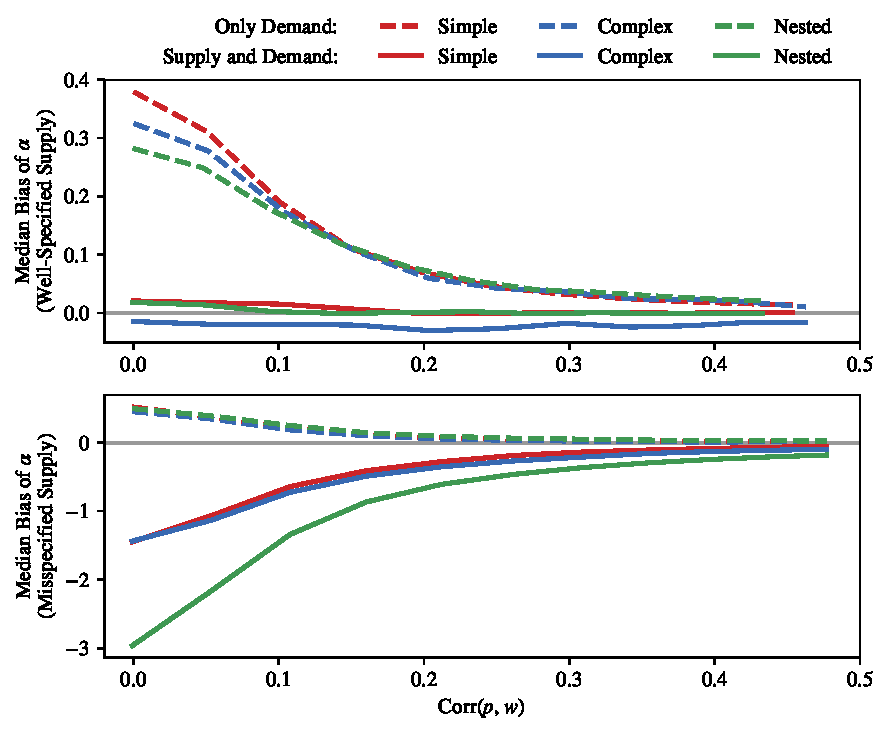
\includegraphics[height=0.95\textheight]{./resources/strength_blp_approximate_bias_alpha_plot.pdf}
\end{center}
\end{frame}


\begin{frame}{What about Hausman Instruments?}
AKA contemporaneous prices of same product in a different market.
\begin{itemize}
    \item Idea is to pick up common cost shocks:
     $$p_{jmt} = c_{jmt} + \eta_{jmt}$$
     \item But this places strong assumptions on nature of demand shocks (and markups $ \eta_{jmt}$)
     \item Even with FE: $\xi_{jmt} = \xi_j + \xi_t + \underbrace{\Delta \xi_{jt}}_{=0} + \Delta \xi_{jmt}$
     \item A common complaint: national advertising might increase demand for a product in multiple geographic markets.
\end{itemize}
\end{frame}



\begin{frame}{Markup Shifters}
The equilibrium markup is a function of \alert{everything!} $\eta_{jt}(\mathbf{p},\mathbf{s},\xi_t,\omega_t,\textrm{x}_{t},\textrm{w}_{t},\textrm{v}_t,\textrm{y}_t,\theta_2)$:
\begin{itemize}
\item It is obviously \alert{endogenous} (depends on error terms)!
\item But lots of potential instruments beyond \alert{excluded} $\textrm{v}_t$ or $\textrm{w}_t$.
\item Idea: cross-market variation in number or strength of competitors
\begin{itemize}
\item Also $\textrm{v}_{-j}$ and $w_{-j}$ and $x_{-j}$.
\item Not $p_{-j}$ or $\xi_{-j}$, etc.
\item The idea is that these instruments shift the \alert{marginal revenue curve}.
\item What is a good choice of $f(x_{-j})$? etc.
\end{itemize}
\end{itemize}
\end{frame}




\begin{frame}{BLP Instruments}
\begin{itemize}
\item Common choices are average characteristics of other products in the same market $f(x_{-j,t})$. \alert{BLP instruments}
\begin{itemize}
\item Same firm $z_{1jt} = \overline{x}_{-j_f,t} = \frac{1}{\left\vert{F_j}\right\vert}  \sum_{k \in \mathcal{F}_j} x_{kt} - \frac{1}{\left\vert{F_j}\right\vert} x_{jt}$.
\item Other firms $z_{2jt}=\overline{x}_{\cdot t} - \overline{x}_{-j_f,t} - \frac{1}{J} x_{jt}$.
\item Plus regressors $(1, x_{jt})$.
\item Plus higher order interactions 
\end{itemize}
\item Technically linearly independent for large (finite) $J$, but becoming highly correlated.
\begin{itemize}
\item Can still exploit variation in number of products per market or number of products per firm.
\end{itemize}
\item Correlated moments $\rightarrow$ ``many instruments''.
\begin{itemize}
\item May be inclined to ``fix'' correlation in instrument matrix directly.
\end{itemize}
\end{itemize}
\end{frame}


\begin{frame}{Armstrong (2016): Weak Instruments?}
Consider the limit as $J \rightarrow \infty$
\begin{eqnarray*}
\frac{s_{jt}(\mathbf{p_t})}{\left|\frac{\partial s_{jt}(\mathbf{p_t})}{\partial p_{jt}}\right|} = \frac{1}{\alpha} \frac{1}{1-s_{jt}} \rightarrow \frac{1}{\alpha}
\end{eqnarray*}
\begin{itemize}
\item Hard to use markup shifting instruments to instrument for a constant.
\item How close to the constant do we get in practice?
\item Average of $x_{-j}$ seems like an especially poor choice. Why?
\item Shows there may still be some power in: products per market, products per firm.
\item Convergence to constant extends to mixed logits (see Gabaix and Laibson 2004).
\item Suggests that you really need cost shifters.
\end{itemize}
\end{frame}


\begin{frame}{Differentiation Instruments: Gandhi Houde (2019)}
\begin{itemize}
\item Also need instruments for the $\Sigma$ or $\sigma$ random coefficient parameters.
\item Instead of average of other characteristics $f(x) = \frac{1}{J-1} \sum_{k \neq j} x_k$, can transform as distance to $x_j$.
\begin{align*}
d_{jt} ^k=  |x_k - x_j |
\end{align*}
\item And use this transformed to construct two kinds of IV (Squared distance, and count of local competitors)
\begin{align*}
DIV_1 &= \sum_{j \in F}  d_{jt}^2,  \quad  \sum_{j \notin F}  d_{jt}^2 \\
DIV_2 &= \sum_{j \in F}  \mathbb{I}[d_{jt} < c]   \quad \sum_{j \notin F}   \mathbb{I}[d_{jt} < c]
\end{align*}
\item They choose $c$ to correspond to one standard deviation of $x$ across markets.
\item Monotonicity?
\end{itemize}
\end{frame}


\begin{frame}{Differentiation Instruments: Gandhi Houde (2019)}
\begin{center}
\includegraphics[height=0.9\textheight]{resources/d_iv1.png}
\end{center}
\end{frame}


\begin{frame}{Intuition from Linear IV (FRAC: Salanie and Wolak)}
Simple case where $\theta_0 = (\beta_0, \pi_0, \sigma_0)'$. A second-order Taylor expansion around $\pi_0 = \sigma_0 = 0$ gives the following linear model with four regressors:
\begin{equation}
    \label{eq:frac}
    \log\frac{\mathcal{S}_{jt}}{\mathcal{S}_{0t}} \approx \beta_0 x_{jt} + \sigma_0^2 a_{jt} + \pi_0 m_t^y x_{jt} + \pi_0^2 v_t^y a_{jt} + \xi_{jt}, \quad a_{jt} = \Big(\frac{x_{jt}}{2} - \sum_{k \in \mathcal{J}_t} \mathcal{S}_{kt} \cdot x_{kt}\Big) \cdot x_{jt}
\end{equation}
\begin{itemize}
    \item $m_t^y = \sum_{i \in \mathcal{I}_t} w_{it} \cdot y_{it}$ is the within-market demographic mean
    \item $v_t^y = \sum_{i \in \mathcal{I}_t} w_{it} \cdot (y_{it} - m_t^y)^2$ is its variance
    \item $a_{jt}$ is an ``artificial regressor'' that reflects within-market differentiation of the product characteristic $x_{jt}$.\\
    \item Linear but we still need an IV for $a_{jt}$.
\end{itemize}
Implemented in Julia by Jimbo Brand  \url{https://github.com/jamesbrandecon/FRAC.jl}
% where $m_t^y = \sum_{i \in \mathcal{I}_t} w_{it} \cdot y_{it}$ is the within-market demographic mean, $v_t^y = \sum_{i \in \mathcal{I}_t} w_{it} \cdot (y_{it} - m_t^y)^2$ is its variance, and $a_{jt}$ is an ``artificial regressor'' that reflects within-market differentiation of the product characteristic $x_{jt}$.\footnote{\cite{salanie2019fast} give additional intuition for the functional form of $a_{jt}$. A quadratic form is unsurprising because $x_{jt}$ multiplied $\nu_{it}$. The $\frac{1}{2}$ comes from the symmetric shape of the logistic distribution.} If $\pi_0 = \sigma_0 = 0$, the approximation is exact, and collapses to a simple logit regression: $\log(\mathcal{S}_{jt} / \mathcal{S}_{0t}) = \delta_{jt} = \beta_0 x_{jt} + \xi_{jt}$.
\end{frame}


\begin{frame}{Connection or when do GH IV work well?}
Recall the GH IV are:
\begin{align*}
J \cdot x_{jt}^2 + \underbrace{\sum_k x_{kt}^2}_{\text{ constant for } t } - 2 \sum_k x_{jt} \cdot x_{kt}
\end{align*}
and the artificial regressor is
\begin{align*}
\frac{1}{2} x_{jt}^2 - 2 x_{jt} \cdot \sum_k \mathcal{S}_{kt}  \cdot x_{kt}
\end{align*}
\begin{itemize}
\item We should be \alert{share weighting} the interaction term, but GH assume equal weighting.\\
\item Should be able to do better than these IV (but ideal is infeasible...)
\item Alternative take: GH propose IIA test that looks a lot like Salanie Wolak estimator. Good for starting values? Or as pre-test for heterogeneity?
\item Warning: I find these are always nearly colinear and run PCA first...
\end{itemize}
\end{frame}


\begin{frame}{Optimal Instruments}
\begin{itemize}
\item Since any $f(x,z)$ satisfies our orthogonality condition, we can try to choose $f(x,z)$ as a \alert{basis} to approximate optimal instruments. (Newey 1990)
\item This is challenging in practice -- and in fact suffers from a curse of dimensionality.
\item This is frequently given as a rationale behind higher order $x$'s.
\item When the dimension of $x$ is low -- this may still be feasible. ($K \leq 3)$.
\end{itemize}
\end{frame}



\begin{frame}{Optimal Instruments (Chamberlain 1987)}
Chamberlain (1987) asks how can we choose $f(z_i)$ to obtain the semi-parametric efficiency bound with conditional moment restrictions:
\begin{align*}
\mathbb{E}[g(z_i,\theta) | z_i]=0 \Rightarrow \mathbb{E}[g(z_i,\theta) \cdot f(z_i) ]=0 
\end{align*}
Recall that the asymptotic GMM variance depends on $(G'\, \Omega^{-1} G\,)$

The answer is to choose instruments related to the (expected) Jacobian of moment conditions w.r.t $\theta$. The true Jacobian at $\theta_0$ is \alert{infeasible}:
\begin{align*}
G=\mathbb{E}\left[\frac{\partial g(z_i,\theta)}{\partial \theta} | z_i, \theta_0 \right]
\end{align*}
%Dominguez and Lobato (2004) point out we can get unlucky and choose an $f(z_i)$ such that $\theta$ is no longer identified(!)
\end{frame}


\begin{frame}{Optimal Instruments (Chamberlain 1987)}
Consider the simplest IV problem:
\begin{align*}
y_i &= \beta x_i + \gamma v_i + u_i \quad \text{ with } \quad \mathbb{E}[u_i | v_i, z_i] =0 \\
u_i &= \left(y_i - \beta x_i - \gamma v_i \right) \\
g(x_i,v_i,z_i) &= \left(y_i - \beta x_i - \gamma v_i \right) \cdot [v_i,\, z_i]
 \end{align*}
 Which gives:
\begin{align*}
\mathbb{E}\left[\frac{\partial g(x_i,v_i, z_i,\theta)}{\partial \gamma} \mid v_i, z_i \right] &\propto v_i\\
\mathbb{E}\left[\frac{\partial g(x_i,v_i, z_i,\theta)}{\partial \beta} \mid v_i, z_i \right] &
\propto \mathbb{E}\left[x_i \mid v_i, z_i \right]
\end{align*}
We can't just use $x_i$ (bc endogenous!), but you can also see where 2SLS comes from...
\end{frame}




\begin{frame}{Optimal Instruments (Newey 1990)}
From previous slide, nothing says that $\mathbb{E}\left[x_i \mid v_i, z_i \right]$ needs to be \alert{linear}!
\begin{itemize}
\item Since any $f(x,z)$ satisfies our orthogonality condition, we can try to choose $f(x,z)$ as a \alert{basis} to approximate optimal instruments.
\item Why? Well affine tranformations of instruments are still valid, and we span the same vector space!
\item We are essentially relying on a non-parametric regression that we never run (but could!)
\begin{itemize}
\item This is challenging in practice -- and in fact suffers from a curse of dimensionality.
\item This is frequently given as a rationale behind higher order $x$'s.
\item When the dimension of $x$ is low -- this may still be feasible. ($K \leq 5)$.
\item But recent improvements in sieves, LASSO, non-parametric regression are encouraging.
\end{itemize}
\end{itemize}
\end{frame}



\begin{frame}{Optimal IV: BLP}
Recall the GMM moment conditions are given by $\mathbb{E}[\xi_{jt} | Z_{jt}^D]=0$ and $\mathbb{E}[\omega_{jt} | Z_{jt}^S]=0$ and the asymptotic GMM variance depends on $(G'\, \Omega^{-1} G\,)$ where the expressions are given below:
\begin{align*}
    G=\mathbb{E}\left[
    \left(\frac{\partial \xi_{jt}}{\partial \theta}, \,
    \frac{\partial \omega_{jt}}{\partial \theta} \right)
| \mathbf{Z_t} \right], \quad 
\Omega = \mathbb{E}\left[
\begin{pmatrix}
    \xi_{jt} \\
    \omega_{jt}
\end{pmatrix}
\begin{pmatrix}
    \xi_{jt}\, \,
    \omega_{jt}
\end{pmatrix}
| \mathbf{Z_t} \right].
\end{align*}
Chamberlain (1987) showed that the approximation to the optimal instruments are given by the expected Jacobian contribution for each observation $(j,t)$: $\mathbb{E}[G_{jt}(\mathbf{Z_t})\, \Omega_{jt}^{-1} | \mathbf{Z_t}]$.\\
\end{frame}




\begin{frame}{Optimal Instruments (see Conlon Gortmaker 2020)}
\noindent BLP 1999 tells us the (Chamberlain 1987) optimal instruments for this supply-demand system of $G\, \Omega^{-1}$ where for a given observation $n$, we need to compute $\mathbb{E}[\frac{\partial \xi_{jt}}{\partial \theta} | \mathbf{Z_t}]$ and $\mathbb{E}[\frac{\partial \omega_{jt}}{\partial \theta} | \mathbf{Z_t}]$

\begin{align*}
    G_{jt} \equiv \underbrace{
        \begin{bmatrix}
            \frac{\partial \xi_{jt}}{\partial \beta}
            & \frac{\partial \omega_{jt}}{\partial \beta} \\
            \frac{\partial \xi_{jt}}{\partial \alpha}
            & \frac{\partial \omega_{jt}}{\partial \alpha} \\
            \frac{\partial \xi_{jt}}{\partial \widetilde{\theta}_2}
            & \frac{\partial \omega_{jt}}{\partial \widetilde{\theta}_2} \\
            \frac{\partial \xi_{jt}}{\partial \gamma} 
            & \frac{\partial \omega_{jt}}{\partial \gamma} 
        \end{bmatrix}
    }_{(K_1 + K_2 + K_3)\times 2}
    = 
    \begin{bmatrix}
        -\mathrm{x}_{jt} & 0 \\
        -\mathrm{v}_{jt} & 0 \\
        \frac{\partial \xi_{jt}}{\partial \alpha}  
        &  \frac{\partial \omega_{jt}}{\partial \alpha}\\
        \frac{\partial \xi_{jt}}{\partial \widetilde{\theta}_2} 
        & \frac{\partial \omega_{jt}}{\partial \widetilde{\theta}_2} \\
        0 & -\mathrm{x}_{jt} \\
        0 & -\mathrm{w}_{jt}
    \end{bmatrix}
    , \quad \Omega_t \equiv 
    \underbrace{
        \begin{bmatrix}
        \sigma^2_{\xi_t} & \sigma_{\xi_t \omega_t}\\
        \sigma_{\xi_t \omega_t} & \sigma^2_{\omega_t}
    \end{bmatrix}
    }_{2 \times 2}.
\end{align*}
\end{frame}


\begin{frame}{Optimal Instruments: (see Conlon Gortmaker 2020) }
\noindent I replace co-linear elements with zeros using $\odot \Theta$
\begin{align*}
    (G_{jt} \Omega_t^{-1} ) \odot \Theta =  \frac{1}{\sigma_\xi^2 \sigma_\omega^2 - \sigma_{\xi \omega}^2} \cdot 
    \begin{bmatrix}
        -\sigma_\omega^2 x_{jt} & 0  \\
        -\sigma_\omega^2 v_{jt} & \sigma_{\xi \omega} v_{jt} \\
        \sigma_\omega^2 \frac{\partial \xi_{jt}}{\partial \alpha} - 
        \sigma_{\xi\omega}\frac{\partial \omega_{jt}}{\partial \alpha} 
        & \sigma_{\xi}^2 \frac{\partial \omega_{jt}}{\partial \alpha}  - 
        \sigma_{\xi\omega}\frac{\partial \xi_{jt}}{\partial \alpha}  \\
        \sigma_\omega^2 \frac{\partial \xi_{jt}}{\partial \widetilde{\theta}_2}  -
        \sigma_{\xi\omega}\frac{\partial \omega_{jt}}{\partial \widetilde{\theta}_2} 
        & \sigma_{\xi}^2 \frac{\partial \omega_{jt}}{\partial \widetilde{\theta}_2} - 
        \sigma_{\xi\omega}\frac{\partial \xi_{jt}}{\partial \widetilde{\theta}_2}\\
        0 &  -\sigma_{\xi}^2 x_{jt} \\
        \sigma_{\xi\omega} w_{jt} & -\sigma_{\xi}^2 w_{jt}
    \end{bmatrix}
    .
\end{align*}
\noindent Now we can partition our instrument set by column into ``demand'' and ``supply'': 
\begin{align*}
    Z_{jt}^{\textit{Opt},D} \equiv \underbrace{\E[(G_{jt}(Z_t) \Omega_t^{-1} \odot \Theta)_{\cdot 1} | \chi_t]}_{K_1 + K_2 + (K_3 - K_x)}, \quad Z_{jt}^{\textit{Opt},S} \equiv \underbrace{\E[(G_{jt}(Z_t)\Omega_t^{-1} \odot \Theta)_{\cdot 2} | \chi_t]}_{K_2 + K_3+ (K_1 - K_x)}.
\end{align*}
\end{frame}


% \begin{frame}{Aside: What does Supply tell us about Demand?}
% \begin{align*}
% & \textbf{Demand} & \textbf{Supply} \\
% \del \alpha:& 
%         \sigma_\omega^2 \frac{\partial \xi_{jt}}{\partial \alpha} - 
%         \sigma_{\xi\omega}\frac{\partial \omega_{jt}}{\partial \alpha} 
%         & \sigma_{\xi}^2 \frac{\partial \omega_{jt}}{\partial \alpha}  - 
%         \sigma_{\xi\omega}\frac{\partial \xi_{jt}}{\partial \alpha}  \\
% \del \sigma:& 
%         \sigma_\omega^2 \frac{\partial \xi_{jt}}{\partial \widetilde{\theta}_2}  -
%         \sigma_{\xi\omega}\frac{\partial \omega_{jt}}{\partial \widetilde{\theta}_2} 
%         & \sigma_{\xi}^2 \frac{\partial \omega_{jt}}{\partial \widetilde{\theta}_2} - 
%         \sigma_{\xi\omega}\frac{\partial \xi_{jt}}{\partial \widetilde{\theta}_2}
% \end{align*}
% \begin{itemize}
% \item These are \alert{cross equation restrictions}
% \item They serve as \alert{overidentifying restrictions} for $\theta_2$ parameters.
% \item This is the what imposing supply side tells us about demand (and \textit{vice versa})
% \end{itemize}
% \end{frame}


\begin{frame}{Optimal Instruments}
How to construct optimal instruments in form of Chamberlain (1987). Start with initial instruments $\chi_t = A\left(\mathbf{X_t},\mathbf{W_t},\mathbf{V_t}\right)$
\begin{eqnarray*}
\mathbb{E}\left[\frac{\partial \xi_{jt}}{\partial \theta} | \chi_{t} \right] = \left[\beta, E\left[\frac{\partial \xi_{jt}}{\partial \alpha} | \chi_{t} \right] ,
 \mathbb{E}\left[\frac{\partial \xi_{jt}}{\partial \widetilde{\theta}_2} | \chi_{t} \right] \right]
\end{eqnarray*}
Some challenges:
\begin{enumerate}
\item $p_{jt}$ or $\eta_{jt}$ depends on $(\omega_{j},\xi_{t})$ in a highly nonlinear way (no explicit solution!).
\item $\mathbb{E}\left[\frac{\partial \xi_{jt}}{\partial \widetilde{\theta}_2} \mid X_t, w_{t} \right] =\mathbb{E}\left[\left[\frac{\partial \mathbf{s_t}}{\partial \mathbf{\delta_t}}\right]^{-1} 
\left[\frac{\partial \mathbf{s_t}}{\partial \widetilde{\theta}_2}\right] \mid Z_{jt}^D \right]$  (not conditioned on endogenous $p$!)
\end{enumerate}
Things are \alert{infeasible} because we don't know $\theta_0$!
\end{frame}


\begin{frame}{Feasible Recipe (BLP 1999)}
\begin{enumerate}
\item Fix $\widehat{\theta}=(\widehat{\theta}_1,\widehat{\theta}_2,\widehat{\theta}_3)$ and draw $(\boldsymbol{\xi}^{*},\boldsymbol{\omega}^{*})$ from empirical density
\item Solve firm FOC's for $\mathbf{\hat{p}_{t}}(\boldsymbol{\xi}^{*},\boldsymbol{\omega}^{*},\widehat{\theta})$
\item Solve shares $\mathbf{s_{t}}(\mathbf{\hat{p}_{t}},\widehat{\theta})$
\item Compute necessary Jacobian
\item Average over multiple values of$(\boldsymbol{\xi}^{*},\boldsymbol{\omega}^{*})$. (Lazy approach: use only $(\boldsymbol{\xi}^{*},\boldsymbol{\omega}^{*})=0$).
\end{enumerate}
In simulation the ``lazy'' approach does just as well. (At least for iid normal $(\boldsymbol{\xi},\boldsymbol{\omega})$)\\

 Alternative: Can we use $\mathbb{E}[ \mathbf{p_t} \mid \mathbf{Z_t}]$ instead for (2) if we don't have supply side
\end{frame}



\begin{frame}{Simplified Version: Reynaert Verboven (2014)}
\begin{itemize}
\footnotesize
\item Optimal instruments are easier to work out if $p = mc$.
\begin{eqnarray*}
c = p  + \underbrace{\Delta^{-1} s}_{\rightarrow 0}  = X \gamma_1 + W \gamma_2 + \omega
\end{eqnarray*}
\item Linear cost function means linear reduced-form price function (could do nonlinear regression too)
\begin{eqnarray*}
E\left[ \frac{\partial \xi_{jt} }{\partial \alpha} | z_t \right] &=& E[p_{jt} | z_t] = x_{jt} \gamma_1 + w_{jt} \gamma_2\\
E\left[ \frac{\partial \omega_{jt} }{\partial \alpha} | z_t \right] &=& 0 , \quad E\left[ \frac{\partial \omega_{jt} }{\partial \widetilde{\theta}_2} | z_t \right] = 0\\
E\left[ \frac{\partial \xi_{jt} }{\partial \widetilde{\theta}_2} | z_t \right] &=&E\left[ \frac{\partial \delta_{jt} }{\partial \widetilde{\theta}_2} | z_t \right]\\
\end{eqnarray*}
\item If we are worried about endogenous oligopoly markups is this a reasonable idea?
\item Turns out that the important piece tends to be \alert{shape} of jacobian for $\sigma_x$.
\item In either case what we care about is $\mathbb{E}[p \mid x, z]$ (the \alert{first stage}). Nothing is free here !
\end{itemize}
\end{frame}

\begin{frame}{Optimal Instruments: Reynaert Verboven (2014)}
\begin{center}
\includegraphics[height=0.9\textheight]{resources/verboven.png}
\end{center}
\end{frame}




\begin{frame}{IV Comparison: Conlon and Gortmaker (2020)}
\begin{center}
\includegraphics[width=4.9in]{resources/inst_table.png}
\end{center}
\end{frame}

\begin{frame}{IV Comparison: Conlon and Gortmaker (2020)}
\begin{center}
\includegraphics[width=3.9in]{resources/fixed_parameters_simple_plot.pdf}
\end{center}
\end{frame}



\begin{frame}{Takeaway}
What does this mean:
\begin{itemize}
    \item We should always check $\mathbb{E}[p \mid x, z]$ before we do anything else.
    \item Can use FRAC to figure out where the heterogeneity is, get startingn values
    \item May want to consider adding a supply side (if you're willing to assume for counterfactuals, why not?)
    \item Certainly should do \texttt{results.compute\_optimal\_instruments()} in PyBLP.
\end{itemize}
\end{frame}


\end{document}